
%\documentclass[12pt,journal,compsoc]{IEEEtran}
%\documentclass[journal]{IEEEtran}  % good for final publication format

%\documentclass[twocolumn]{IEEEtran} %!PN
%\documentclass[draftcls]{IEEEtran} % good for double space and two columns!PN

%\documentclass[draftcls, onecolumn]{IEEEtran} % good for submission with double space
\documentclass[onecolumn]{IEEEtran} % good for a report with a single space!
%
% If IEEEtran.cls has not been installed into the LaTeX system files,
% manually specify the path to it like:
% \documentclass[journal]{../sty/IEEEtran}

% *** CITATION PACKAGES ***
%
\usepackage{cite}

\usepackage{color}
\definecolor{red}{rgb}{1,0,0}
% textcolor{text}

% *** GRAPHICS RELATED PACKAGES ***
%
\ifCLASSINFOpdf
  \usepackage[pdftex]{graphicx}
  % declare the path(s) where your graphic files are
  % \graphicspath{{../pdf/}{../jpeg/}}
  % and their extensions so you won't have to specify these with
  % every instance of \includegraphics
  % \DeclareGraphicsExtensions{.pdf,.jpeg,.png}
\else
  % or other class option (dvipsone, dvipdf, if not using dvips). graphicx
  % will default to the driver specified in the system graphics.cfg if no
  % driver is specified.
  % \usepackage[dvips]{graphicx}
  % declare the path(s) where your graphic files are
  % \graphicspath{{../eps/}}
  % and their extensions so you won't have to specify these with
  % every instance of \includegraphics
  % \DeclareGraphicsExtensions{.eps}
\fi

% *** MATH PACKAGES ***
\usepackage{amssymb}
\usepackage[cmex10]{amsmath}
\usepackage{amsfonts}

% *** ALIGNMENT PACKAGES ***
\usepackage{array}

% *** SUBFIGURE PACKAGES ***
%\ifCLASSOPTIONcompsoc
%  \usepackage[caption=false,font=uniformsize,labelfont=sf,textfont=sf]{subfig}
%\else
%  \usepackage[caption=false,font=footnotesize]{subfig}
%\fi

\usepackage{subfigure}

% *** FLOAT PACKAGES ***
\usepackage{dblfloatfix}

%\ifCLASSOPTIONcaptionsoff
%  \usepackage[nomarkers]{endfloat}
% \let\MYoriglatexcaption\caption
% \renewcommand{\caption}[2][\relax]{\MYoriglatexcaption[#2]{#2}}
%\fi
% endfloat.sty was written by James Darrell McCauley, Jeff Goldberg and
% Axel Sommerfeldt. This package may be useful when used in conjunction with
% IEEEtran.cls'  captionsoff option. Some IEEE journals/societies require that
% submissions have lists of figures/tables at the end of the paper and that
% figures/tables without any captions are placed on a page by themselves at
% the end of the document. If needed, the draftcls IEEEtran class option or
% \CLASSINPUTbaselinestretch interface can be used to increase the line
% spacing as well. Be sure and use the nomarkers option of endfloat to
% prevent endfloat from "marking" where the figures would have been placed
% in the text. The two hack lines of code above are a slight modification of
% that suggested by in the endfloat docs (section 8.4.1) to ensure that
% the full captions always appear in the list of figures/tables - even if
% the user used the short optional argument of \caption[]{}.
% IEEE papers do not typically make use of \caption[]'s optional argument,
% so this should not be an issue. A similar trick can be used to disable
% captions of packages such as subfig.sty that lack options to turn off
% the subcaptions:
% For subfig.sty:
% \let\MYorigsubfloat\subfloat
% \renewcommand{\subfloat}[2][\relax]{\MYorigsubfloat[]{#2}}
% However, the above trick will not work if both optional arguments of
% the \subfloat command are used. Furthermore, there needs to be a
% description of each subfigure *somewhere* and endfloat does not add
% subfigure captions to its list of figures. Thus, the best approach is to
% avoid the use of subfigure captions (many IEEE journals avoid them anyway)
% and instead reference/explain all the subfigures within the main caption.
% The latest version of endfloat.sty and its documentation can obtained at:
% http://www.ctan.org/tex-archive/macros/latex/contrib/endfloat/
%
% The IEEEtran \ifCLASSOPTIONcaptionsoff conditional can also be used
% later in the document, say, to conditionally put the References on a
% page by themselves.

% correct bad hyphenation here
\hyphenation{op-tical net-works semi-conduc-tor}

%%%%%%%%%%%%%%%%%%%%%%%%%%%%%%%%%%%%%%%%%%%%%%%%%%%%%%%%%%%%%%%%%%%%%
%%%%%%%%%%%%%%%%%%%%%%%%%%%%%%%%%%%%%%%%%%%%%%%%%%%%%%%%%%%%%%%%%%%%%
%                               BEGIN DOCUMENT
%%%%%%%%%%%%%%%%%%%%%%%%%%%%%%%%%%%%%%%%%%%%%%%%%%%%%%%%%%%%%%%%%%%%%
%%%%%%%%%%%%%%%%%%%%%%%%%%%%%%%%%%%%%%%%%%%%%%%%%%%%%%%%%%%%%%%%%%%%%

\begin{document}
%
% paper title
% Titles are generally capitalized except for words such as a, an, and, as,
% at, but, by, for, in, nor, of, on, or, the, to and up, which are usually
% not capitalized unless they are the first or last word of the title.
% Linebreaks \\ can be used within to get better formatting as desired.
% Do not put math or special symbols in the title.
\title{Transient VRM Response from a Large Circular Loop over a Conductive and Magnetically Viscous Half-Space}

%=======================================================
%=======================================================
%                       AUTHORS
%=======================================================
%=======================================================

% \author{Devin Cowan, {\it Student Member, IEEE}, Lin-Ping Song, {\it Member, IEEE}, and Douglas W. Oldenburg
% \thanks{Devin Cowan, Lin-Ping Song and Douglas W. Oldenburg
% are with the University of British Columbia Department of Earth, Ocean and Atmospheric Sciences, Vancouver, BC, Canada.}
% \thanks{The corresponding author on this paper is Devin Cowan, Email: devinccowan@gmail.com}
% }



% The paper headers
% \markboth{IEEE TRANSACTIONS ON GEOSCIENCE AND REMOTE SENSING. }%
% {Shell \MakeLowercase{\textit{et al.}}: Bare Demo of IEEEtran.cls for Journals}

% make the title area
\maketitle

%=======================================================
%=======================================================
%               ABSTRACT
%=======================================================
%=======================================================

\begin{abstract}
To effectively characterize the impact of viscous remanent magnetization (VRM) on the transient electromagnetic response, we present a set of analytical expressions for the vertical and  radial VRM responses generated by a large circular loop over a magnetically viscous half-space.  For a step-off excitation, N\'{e}el relaxation theory is used to express the VRM within the half-space as the product of a static on-time magnetization and a time-dependent after-effect function. Through heuristic and empirical approximations to the elliptic integral of the second kind, we are able to convert Hankel  integral-based expressions for static fields into simplified  analytical expressions. These were validated with a numerical 1D forward modelling code. Analytical expressions show that VRM responses are largest near the transmitter  wire, and that at the centre of a large loop, the strength of the VRM response is inversely proportional to the loop's radius. We also present an estimate of the cross-over time from which the VRM signal starts to dominate the transient response. We found that later cross-over times were observed near the centers of large loops and that cross-over times were much earlier near the transmitter wire. Also, the magnetic flux density has an earlier cross-over time compared to its time derivative. To lower or remove the VRM response in an anticipated survey, our analytical expressions can be used straightforwardly to choose an appropriate loop size, identify the VRM response time window, and select an optimal set of time channels.

\end{abstract}

% Note that keywords are not uniformly used for peerreview papers.
%{\bf Keywords:} Viscous remanent magnetization, magnetic soil, inductive response, a circular loop, cross-over time, TEM systems.


%=======================================================
%=======================================================
%               INTRODUCTION
%=======================================================
%=======================================================

\section{Introduction}
Many inductive source time-domain electromagnetic (TEM) systems use a step-off like excitation to measure the response from a desired target. In lateritic soils, sudden removal of the transmitter's primary field induces a time-dependent magnetic relaxation due to the presence of superparamagnetic (SP) iron-oxide grains \citep{Buselli1982, Barsukov2001,Billings2003,Pasion2007,Zadorozhnaya2012}. This magnetic relaxation process is known as viscous remanent magnetization (VRM), magnetic viscosity or magnetic after-effect \citep{Dabas1992,Neel1949,Moskowitz1985}. The VRM experienced by a lateritic soil generates a distinct transient response from that of a non-magnetic conductive soil. This response, termed the VRM response, can severely contaminate the TEM responses from conductive ore bodies and unexploded ordnance items when lateritic soils are prominent \citep{Butler2003, Billings2003,Pasion2007,Buselli1982,Barsukov2001,Zadorozhnaya2012}. Thus to properly account for the VRM signal in a set of TEM data, it is of practical interest to first understand the behaviours of the VRM response.

Over the past decades, studies have been done to characterize the VRM responses exhibited by magnetically viscous soils \citep{Pasion2002, Butler2003, Billings2003,Pasion2007,Buselli1982,Barsukov2001,Zadorozhnaya2012}.  It is well-known that the induced voltage within a receiver coil due to the VRM  response has a $1/t$ decay, where $t$ is the time. Through experimental, analytical and numerical means, researchers have also shown  that measured VRM responses can be diminished by: separating the receiver from the transmitter, increasing the size of the transmitter loop, or elevating the sensor further above the ground \citep{Lee1984, Buselli1982, Barsukov2001, Das2006, Kozhevnikov2007, Zadorozhnaya2012}. Despite providing significant insight, some details regarding the VRM response and its computation appear elusive. Existing numerical and analytical methods \citep{Billings2003, Kozhevnikov2007, Pasion2007, Barsukov2001,Das2004, Druyts2009, Lee1984, Das2006} are both complicated and lack  sufficient insight regarding the quantitative dependence of the VRM  response on the survey geometry. In addition, the current understanding of the VRM response is mainly drawn from the vertical component. With the increasing development of advanced tri-axial TEM sensors, characterizing the radial VRM response is another necessary and desirable aspect.

In this paper, we attempt to fill gaps left in previous studies of the VRM response. We consider a circular transmitter loop over a magnetically viscous half-space and derive simplified analytical expressions for the vertical and horizontal components of the VRM response. Both the magnetic flux and its time derivative are considered for several survey configurations. With the set of new formulae, we are able to effectively model the transient VRM response directly as a function of the survey's geometric properties and predict the times when the VRM signal dominates the TEM response. As a result, quantitative information can easily be obtained to characterize the amplitude and time range of transient VRM responses.

The remainder of this paper is organized as follows. In section II, we review N\'{e}el relaxation theory in the frequency and time domain. General formulation of the VRM response is briefly presented in Section III. In section IV, we derive the analytical expressions for vertical and radial static magnetic fields over a superparamagnetic half-space. These are used to predict the VRM response in Section V, where final analytical expressions are validated using a 1D numerical modeling code. In section VI, we inspect the separability of inductive and VRM responses over a conductive and magnetically viscous half-space and present the analytical formulae to estimate the cross-over time. Section VII concludes the paper.




%==========================================
%==========================================
%       NEW SECTION: VRM RESPONSE GENERAL
%==========================================
%==========================================

\section{Magnetic Viscosity in Lateritic Soils: A Review of N\'{e}el Relaxation Theory}
\label{secAfterEffect}
The magnetic viscosity observed in lateritic soils is commonly understood using thermal relaxation models \citep{Neel1949} for a collection of non-interacting SP single-domain grains \citep{Buselli1982,Moskowitz1985,Dabas1992,Pasion2002,Billings2003,Pasion2007}. In this section, we present mathematical expressions derived by \cite{Neel1949} that will be used later to predict the VRM response for a half-space.

%==========================================
%       SUBSECTION: MAGNETIC SUSCEPTIBILITY
%==========================================
\subsection{Frequency-Dependent Magnetic Susceptibility}
Magnetic susceptibility relates the induced magnetization $\vec M (\omega)$ to the applied magnetic field $\vec H (\omega)$. For  lateritic soils, the magnetic susceptibility can be frequency-dependent \citep{Lee1984,Dabas1992,Fannin1995}:
\begin{equation}
\vec M(\omega) = \chi (\omega) \vec H (\omega).
\end{equation}
By assuming that all SP grains are identical, the frequency-dependent magnetic susceptibility for a theoretical sample can be expressed using a Debye model \citep{Dabas1992,Mullins1973,Pasion2007}:
\begin{equation}
\chi(\omega) = \chi_\infty + \frac{\Delta \chi}{1 + i\omega \tau},
\label{eqChiOmegaDebye}
\end{equation}
where $\tau$ is the time-relaxation constant for the collection of SP grains, $\Delta \chi$ represents the variation in magnetic susceptibility over $\omega \in [0, \infty ]$ due to viscous remanent magnetization, and $\chi_\infty$ is the susceptibility representing instantaneous magnetization within the sample. The time-relaxation constant for the sample is given by \cite{Neel1949}:
\begin{equation}
\tau =  \tau_0 \; \exp \Bigg ( \frac{E_b}{k_B T} \Bigg ),
\label{eqNeelRelaxationTime}
\end{equation}
where $k_B$ is the Boltzmann constant, $T$ is the absolute temperature, and $\tau_0 \sim 10^{-9}$ s is the "attempt time". $E_b$ represents the energy barriers that maintain the pre-existing orientations of individual SP grains. In natural soils, $E_b$ is not the same for all SP grains, and instead forms a distribution. By Eq. (\ref{eqNeelRelaxationTime}), lateritic soils are characterized by a distribution of time-relaxation constants that is represented using a weighting function $f(\tau)$. Applying the weighting function and integrating over all Debye models (\ref{eqChiOmegaDebye}), the soil's magnetic susceptibility is expressed as \citep{Dabas1992,Mullins1973,Pasion2007}:
\begin{equation}
\chi(\omega) = \chi_\infty + \Delta \chi \int_0^\infty \frac{f(\tau)}{1 + i \omega \tau} d\tau
\label{eqChiWeightedIntegral}
\end{equation}

The majority of lateritic soil samples can be adequately fit by assuming a log-uniform distribution of time-relaxation constants between a set of finite limits $[\tau_1, \tau_2]$ \citep{Dabas1992,Mullins1973,Worm1998,Igel2012}. The weighting function for a log-uniform distribution of time-relaxation constants is defined by \citep{Dabas1992,Mullins1973,Billings2003,Das2006}:
\begin{equation}
\label{eqLogDistribution}
f({\tau}) =
\begin{cases}
\dfrac{1}{\tau \; \ln(\tau_2/\tau_1)} & \textrm{for} \; \; \; \tau_1 \leq \tau \leq \tau_2 \\
\; \; \; \; \; \; \; \; \; 0 & \textrm{otherwise}
\end{cases}
\end{equation}
Substituting Eq. (\ref{eqLogDistribution}) into Eq. (\ref{eqChiWeightedIntegral}), we obtain:
\begin{equation}
\begin{split}
\chi (\omega) & = \chi_\infty + \frac{\Delta \chi}{\ln (\tau_2 /\tau_1)} \int_{\tau_1}^{\tau_2} \frac{1}{\tau (1 + i\omega \tau)} d\tau  \\
&= \chi_\infty + \Delta \chi \Bigg [ 1 - \frac{1}{\ln
(\tau_2/\tau_1)} \ln \Bigg ( \frac{1 + i\omega\tau_2}{1 +
i\omega\tau_1} \Bigg ) \Bigg ].
\end{split}
 \label{eqChiOmega}
\end{equation}
Eq. (\ref{eqChiOmega}) represents an appropriate frequency-dependent magnetic susceptibility model that can be used to characterize most lateritic soils \cite{Mullins1973,Lee1984,Worm1998,Dabas1992,Pasion2007}. This model is used to characterize magnetic viscosity in the 1D numerical modeling code \cite{EM1DTM}. It is easy to show, from Eq. (\ref{eqChiOmega}), that $\chi (\omega \rightarrow 0) = \chi_\infty + \Delta \chi$, and that $\chi (\omega\rightarrow \infty) = \chi_\infty$. Thus $\Delta \chi$ represents the static magnetic susceptibility for the collection of SP grains. In this paper, $\chi_\infty$ will not play any significant role when predicting the soil's response as observations will be made during the off-time.


%==========================================
%       SUBSECTION: TRANSIENT MAGNETIZATION
%==========================================

\subsection{Viscous Remanent Magnetization in Response to Step-Off Excitation}

Consider a step-off excitation where a DC field $\vec H_0$, which has been applied to a magnetically viscous sample since $t = -\infty$, is suddenly removed at $t=0$. In this case, the resulting magnetic relaxation at $t >0$ can be expressed as \citep{Neel1949,Billings2003,Pasion2007}:
\begin{equation}
\vec M(t) = \Delta \chi \vec H_0 F(t)
\label{eqMagSte}
\end{equation}
where $F(t)$ is referred to as the after-effect function. If all SP grains are characterized by an identical time-relaxation constant $\tau$, then the after-effect function is given by \citep{Neel1949,Billings2003,Pasion2007}:
\begin{equation}
F (t) = e^{-t/\tau}. \label{afterEffect1}
\end{equation}
For a distribution of time-relaxation constants, Eq. (\ref{afterEffect1}) becomes \citep{Neel1949,Mullins1973,Billings2003,Pasion2007}:
\begin{equation}
\label{eqWeightedIntegral} F(t) = \int^{\infty}_0 f(\tau)
e^{-t/\tau} d \tau,
\end{equation}
where $f(\tau)$ is the weighting function defined in Eq. (\ref{eqChiWeightedIntegral}). For a soil characterized by a log-uniform distribution of time-relaxation constants, substituting Eq. (\ref{eqLogDistribution}) into Eq. (\ref{eqWeightedIntegral}) leads to
\begin{equation}
\begin{split}
F(t) &= \frac{1}{\ln(\tau_2/\tau_1)} \int^{\tau_2}_{\tau_1} \frac{1}{\tau} e^{-t/\tau} d \tau \\
& = \frac{1}{\ln(\tau_2/\tau_1)} \Bigg [ Ei \Big ( \frac{t}{\tau_2} \Big ) - Ei \Big ( \frac{t}{\tau_1} \Big ) \Bigg ],
\end{split}
\label{eqIntDist}
\end{equation}
where $Ei$ is the  exponential integral function. When observations are made at time $\tau_1 \ll t \ll \tau_2$, $Ei (t/\tau_1) \approx
0$ and $Ei (t/\tau_2) \approx -\gamma - \ln(t/\tau_2)$; where $\gamma \approx 0.5772$ is the Euler constant \cite{Pasion2007}. Over this time period, the after-effect function can be approximated by:
\begin{equation}
\label{eqAfterEffectB} F(t) \approx \bar F(t) = \frac{1}{\ln(\tau_2/\tau_1)} \big [ - \gamma - \ln(t) + \ln(\tau_2) \big ].
\end{equation}
%Expression (\ref{eqAfterEffectB}) shows that  viscous remanent
%magnetization in response to a step-off excitation is proportional
%to $\ln(t)$ for $\tau_1 \ll t \ll \tau_2$.
By taking the derivative of Eq. (\ref{eqIntDist}), we obtain
\begin{align}
\label{eqAfterEffectdBdt1}
\frac{d F(t)}{dt} &= \frac{1}{\ln(\tau_2/\tau_1)} \int^{\tau_2}_{\tau_1} - \frac{1}{\tau^2} e^{-t/\tau} d \tau \nonumber \\
& = \frac{1}{\ln(\tau_2/\tau_1)} \Bigg [ \frac{e^{-t/\tau_1} -e^{-t/\tau_2} }{t} \Bigg ].
\end{align}
At time $\tau_1 \ll t \ll \tau_2$, Eq. (\ref{eqAfterEffectdBdt1}) simplifies to the following expression:
\begin{equation}
\label{eqAfterEffectdBdt}
\frac{dF(t)}{d t} \approx \frac{d \bar F(t)}{d t} = -\frac{1}{\ln(\tau_2/\tau_1)} \frac{1}{t}.
\end{equation}
We see that Eqs. (\ref{eqAfterEffectB}) and (\ref{eqAfterEffectdBdt}) describe the transient viscous remanent magnetization and its time derivative as decaying proportional to $\ln(t)$ and $1/t$ for $\tau_1 \ll t \ll \tau_2$, respectively. The $1/t$ dependence is often observed in magnetic soil environments when $\partial B/\partial t$ is being measured \cite{Dabas1992,Buselli1982,Pasion2007}. In sections \ref{secMagnetostatic}, \ref{secVRMresponseFinal} and \ref{secEMversusVRM}, approximate time functions are used to derive the expressions which characterize the viscous remanent magnetization of our half-space to step-off excitation.



%==================================================================
%==================================================================
%       NEW SECTION: VRM RESPONSE IN THE ABSENCE OF SELF-DEMAGNETIZATION
%==================================================================
%==================================================================

\section{General Formulation of the VRM Response in the Absence of Self-Demagnetization}
\label{secSelfDemag}

In the absence of self-demagnetization,  the magnetic anomaly observed outside a magnetized body can be expressed using the following dyadic Green's function \citep{Blakely1996}:
\begin{equation}
\vec B(\vec r,t) = \frac{\mu_0}{4 \pi} \int_{V} \nabla \nabla \frac{1}{| \vec r - \vec r_s |} \cdot \vec M(\vec r_s, t) \, dV_s
\label{Bfield}
\end{equation}
where $r$ is the location of observation, $r_s$ are locations within the volume being integrated, and $t$ represents time.
\\

For a step-off excitation, we can use Eq. (\ref{eqMagSte})  to represent the total magnetization at any location within a magnetically viscous Earth at $t > 0$. This is because any instantaneous magnetization attributed to $\chi_\infty$ is zero during the off-time. In most cases, we can expect $\Delta \chi(\vec r_s)$ and the inducing field $\vec H_0(\vec r_s)$ to varyspatially. If the spatial distribution of time-relaxation constants defined in expression (\ref{eqLogDistribution}) is uniform everywhere within the magnetically viscous Earth, the after-effect function $F(t)$ is spatially invariant and can be taken outside of the integral in Eq. (\ref{Bfield}), which becomes
\begin{align}
\vec B(\vec r,t) &= \frac{\mu_0}{4 \pi} F(t) \int_V \nabla \nabla \frac{1}{| \vec r - \vec r_s |} \cdot \Delta \chi(\vec r_s) \, \vec H_0(\vec r_s) \, dV \nonumber \\
&= \vec B^{(0)} (\vec r) F(t),
\label{eqGenVRMB}
\end{align}
where $\vec B^{(0)}(\vec r)$ defines  the static magnetic response of all SP grains.
\\\\
By taking the derivative of Eq. (\ref{eqGenVRMB}):
\begin{align}
\frac{\partial \vec B(\vec r,t)}{\partial t} &= \frac{\mu_0}{4 \pi} \frac{d F(t)}{dt} \int_V \nabla \nabla \frac{1}{| \vec r - \vec r_s |} \cdot \Delta \chi(\vec r_s) \, \vec H_0(\vec r_s) \, dV \nonumber \\
&= \vec B^{(0)} (\vec r) \frac{d F(t)}{dt}.
\label{eqGenVRMdBdt}
\end{align}
Thus if $\vec B^{(0)}(\vec r)$ is known, the pairs of Eqs. (\ref{eqIntDist}) and (\ref{eqGenVRMB}), Eqs. (\ref{eqAfterEffectdBdt1}) and (\ref{eqGenVRMdBdt}) can be used to predict $\vec B(\vec r,t)$ and $\frac{\partial \vec B(\vec r,t)}{\partial t}$ for the VRM response at $t > 0$. Next we present analytic expressions for $\vec B^{(0)} (\vec r)$.

%============================================================
%============================================================
%       NEW SECTION: DERIVING MAGNETOSTATIC RESPONSE
%============================================================
%============================================================

\section{Deriving the Static Magnetic fields over a Superparamagnetic Half-Space}
\label{secMagnetostatic}

We consider a superparamagnetic half-space in which $\chi_\infty = 0$ in Eq. (\ref{eqChiOmega}).  According to Eqs. (4.87) and (4.88) in \cite{Ward1988}, for a circular transmitter loop with radius of $a$ and at height $h$ above the surface, vertical and radial components of $\vec B^{(0)} (\vec r)$ can be obtained by taking their limits as $\omega \rightarrow 0$, i.e.,
\begin{equation}
\label{eqBzMagnetostatic} B_z^{(0)}(\rho,z) \! = \! \frac{\mu_0 Ia}{2}
\Bigg ( \frac{\Delta \chi}{2+\Delta \chi} \Bigg ) \!\!
\int^{\infty}_0 \!\!\! \lambda e^{-\lambda (z+h)} J_1(\lambda a) J_0
(\lambda \rho) d \lambda
\end{equation}
and
\begin{equation}
\label{eqBrhoMagnetostatic}
B^{(0)}_\rho (\rho,z) \! = \! -\frac{\mu_0 Ia}{2} \Bigg ( \frac{\Delta \chi}{2+\Delta \chi} \Bigg ) \!\!
\int^{\infty}_0 \!\!\! \lambda e^{-\lambda (z+h)} J_1(\lambda a) J_1 (\lambda \rho) d \lambda,
\end{equation}
where $I$ is the steady-state current, $\Delta \chi$ is the static magnetic susceptibility due to the SP effects of the half-space,  $\mu_0 = 4\pi \times 10^{-7}$ H/m is the permeability of free-space, $\rho$ is the radial distance from the loop's center axis, and $z$ is the observation height above the surface. $J_0(\cdot)$ and $J_1(\cdot)$ are 0\textsuperscript{th} and 1\textsuperscript{st} order Bessel functions of the first kind, respectively. Note that we are neglecting the primary field contributions for equations found in \cite{Ward1988}.

We see that even for the static case, the vertical and radial components of $\vec B^{(0)}(\vec r)$ involve solutions to complicated Hankel transforms in Eqs. (\ref{eqBzMagnetostatic}) and (\ref{eqBrhoMagnetostatic}). Their general solutions have to be obtained via numerical integrations \citep{vanDam2004, vanDam2005}. However, for several cases of interest considered in sections \ref{secVertical} and \ref{secRadial}, we can derive analytic solutions or approximate solutions for both the vertical component $B_z(\rho,z)$ and radial component $B_\rho (\rho,z)$.


%============================================================
%       NEW SUBSECTION: VERTICAL MAGNETOSTATIC RESPONSE
%============================================================

\subsection{Vertical Static Response for a Circular Transmitter Loop over a Superparamagnetic Half-space} \label{secVertical} To solve the integral in Eq. (\ref{eqBzMagnetostatic}), we introduce the following identity \citep{Erdelyi1954}:
\begin{equation}
\begin{split}
\int^{\infty}_0 \lambda &e^{-\lambda (z+h)} J_1(\lambda a) J_0 (\lambda \rho) d \lambda \\
&= \frac{a}{\pi} \int_0^\pi \big [ (z +h + i\rho cos\phi )^2 + a^2 \big ]^{-3/2} d\phi
\end{split}.
\label{eqIntSolJ1J0}
\end{equation}
A general analytical solution to Eq. (\ref{eqIntSolJ1J0}) is difficult to derive. For several special cases however, working with the right-hand side of the equation enables us to obtain some insightful field expressions.
\\\\
\subsubsection{Large Circular Loop on the Earth's Surface ($h=0$)}
Assume that the static response is examined close to the Earth's surface ($z \rightarrow 0$). With Wolfram Mathematica's online integration code \citep{Wolfram2016}, the right-hand side of Eq. (\ref{eqIntSolJ1J0}) for $h,z = 0$ can be expressed analytically, i.e.,
\begin{align}
\lim_{z \rightarrow 0} \int^{\infty}_0 \lambda e^{-\lambda z} &J_1(\lambda a) J_0 (\lambda \rho) d \lambda \nonumber \\
\label{eqIntSolJ1J0b} &= \frac{2 }{\pi a} \frac{1}{\sqrt{a^2-\rho^2}} E \Bigg [ \frac{\rho^2}{\rho^2 - a^2} \Bigg ],
\end{align}
where $E[x]$ is the complete elliptic integral of the second kind. Substituting Eq. (\ref{eqIntSolJ1J0b}) into Eq. (\ref{eqBzMagnetostatic}), we have the vertical static response on the Earth's surface at radial distance $\rho$ from the loop's center axis:
\begin{equation}
\begin{split}
B^{(0)}_z(\rho,0) &= \frac{\mu_0 I}{\pi} \Bigg ( \frac{\Delta \chi}{2+\Delta \chi} \Bigg ) \frac{1}{\sqrt{a^2 -\rho^2}} E \Bigg [ \frac{ \rho^2}{\rho^2 - a^2} \Bigg ] \\
&= B^{(0)}_z(0,0) \Bigg ( \frac{2 }{\pi \sqrt{1 -\big ( \frac{\rho}{a} \big )^2}} E \Bigg [ \frac{ \big (\frac{\rho}{a} \big )^2}{\big (\frac{\rho}{a} \big )^2 - 1} \Bigg ] \Bigg ) \\
&= B_z^{(0)}(0,0) \, G \Big (\frac{\rho}{a} \Big ),
\end{split}
\label{eqIntSolJ1J0a3}
\end{equation}
where $B^{(0)}_z (0, 0)$  represents the static magnetic response of the SP half-space at the loop's center, and $G$ is a function that depends explicitly on $(\rho /a)$.
\\


%---------------------------------------
%       FIGURE
%---------------------------------------
\begin{figure}[!t]
\centering
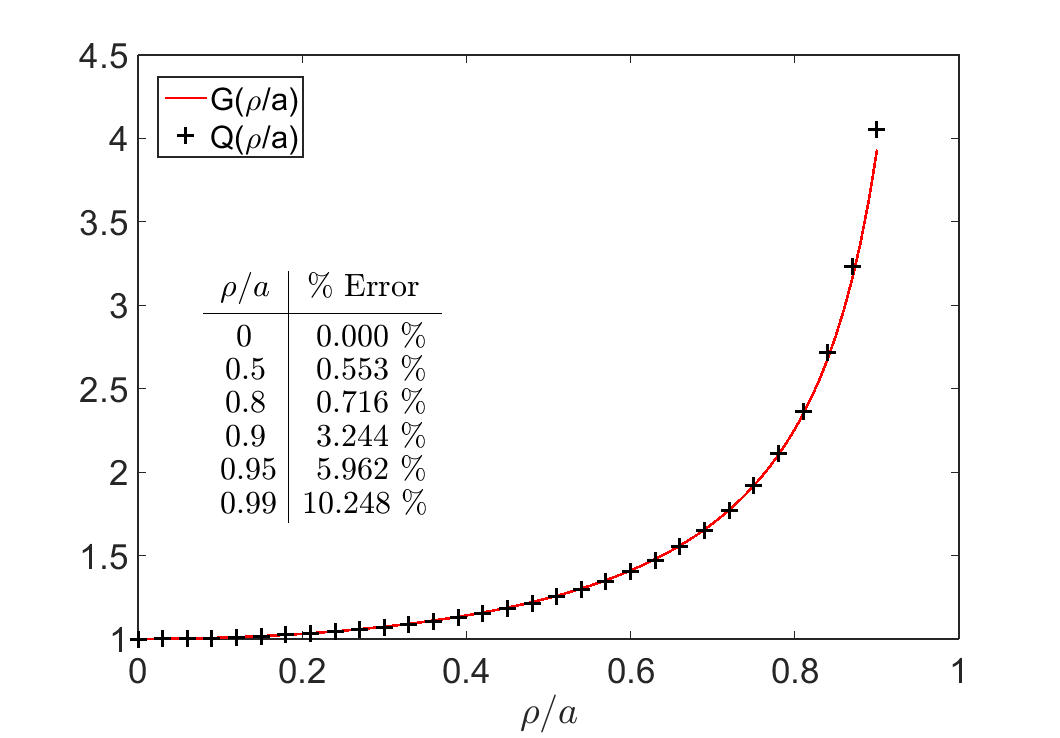
\includegraphics[width=0.50\textwidth]{DCowanVRM2017/imagesColor/figElliptic.png}
\caption{Comaparisson between $G(\rho /a)$  and its approximation $Q(\rho /a)$, for various values of $\rho /a < 1$. A
\% error for selected values is provided.}
\label{figElliptic}
\end{figure}
%---------------------------------------
%
%---------------------------------------

For measurements inside the loop ($\rho <a$), we would like to find an approximate solution for $G$ that does not contain the elliptic integral. At the center of the loop, $\rho /a =0$, $E[0]= \pi /2$, Eq. (\ref{eqIntSolJ1J0a3}) then simplifies to $B_z^{(0)} (0,0)$ as expected. As $\rho \rightarrow a$, the static response approaches infinity. To preserve these properties, we suggest an empirical function $Q$ as:
\begin{equation}
\label{eqElliptic} G \Big ( \frac{\rho}{a} \Big ) \approx Q \Big (
\frac{\rho}{a} \Big ) = 1 + \frac{9}{4\pi} \Bigg ( \frac{\big(
\frac{\rho}{a} \big )^2}{1- \big( \frac{\rho}{a} \big )^2} \Bigg )
\; \; for \; \; \rho < a.
\end{equation}
This approximation  is accurate to within $1\% $ for values $\rho / a \leq 0.8$. For $\rho /a > 0.8$, the approximation increasingly overestimates $Q (\rho /a)$ (Fig. \ref{figElliptic}). Combining Eq. (\ref{eqIntSolJ1J0a3}) with (\ref{eqElliptic}), we have the analytical formula for the vertical static response at any location $(\rho < a,z=0)$ for a loop located on the Earth surface ($h=0$),
\begin{equation}
B^{(0)}_z(\rho,0) \approx \frac{\mu_0 I}{2a}  \Bigg ( \frac{\Delta
\chi}{2+\Delta \chi} \Bigg ) \Bigg [ 1 + \frac{9}{4\pi} \Bigg (
\frac{\big( \frac{\rho}{a} \big )^2}{1- \big( \frac{\rho}{a} \big
)^2} \Bigg ) \Bigg ]. \label{eqStaticLoopBz}
\end{equation}
\\\\

\subsubsection{Response Along the Transmitter's Vertical Axis ($\rho = 0$)} When the transmitter loop is at height $h$ and the observation is along the vertical axis of the transmitter, i.e., at $(\rho =0, z)$, the associated integral in Eq. (\ref{eqIntSolJ1J0}) is reduced to an analytical expression by setting $\rho \rightarrow 0$:
\begin{equation}
\lim_{\rho \rightarrow 0} \int^{\infty}_0 \!\!\! \lambda e^{-\lambda
(z+h)} J_1(\lambda a) J_0 (\lambda \rho) d \lambda \! = \! a \Bigg (
\! \frac{1}{(z+h)^2 + a^2} \! \Bigg )^{3/2}.
\label{eqHankelSolCoin}
\end{equation}
Substituting Eq. (\ref{eqHankelSolCoin}) into Eq. (\ref{eqBzMagnetostatic}) leads to the vertical static response
%\begin{equation}
%B_z(0,z) = \frac{\mu_0 I a^2}{2} \Bigg ( \frac{\Delta \chi}{2 + \Delta \chi} \Bigg ) \Bigg ( \frac{1}{(z+h)^2 + a^2} \Bigg )^{3/2}
%\label{eqStaticDipBz}
%\end{equation}
\begin{equation}
\label{eqStaticCoinBz}
B_z^{(0)}(0,z) = \frac{\mu_0 m}{2 \pi} \Bigg ( \frac{\Delta \chi}{2 + \Delta \chi} \Bigg ) \Bigg ( \frac{1}{(z+h)^2 + a^2} \Bigg )^{3/2},
\end{equation}
where $m=\pi a^2 I$ is the dipole moment of the transmitter.

%============================================================
%       NEW SUBSECTION: RADIAL MAGNETOSTATIC RESPONSE
%============================================================

\subsection{Radial Static Response for a Large Circular Transmitter Loop over a SP Half-space}
\label{secRadial}

%---------------------------------------
%       FIGURE
%---------------------------------------
\begin{figure}[!b]
\centering
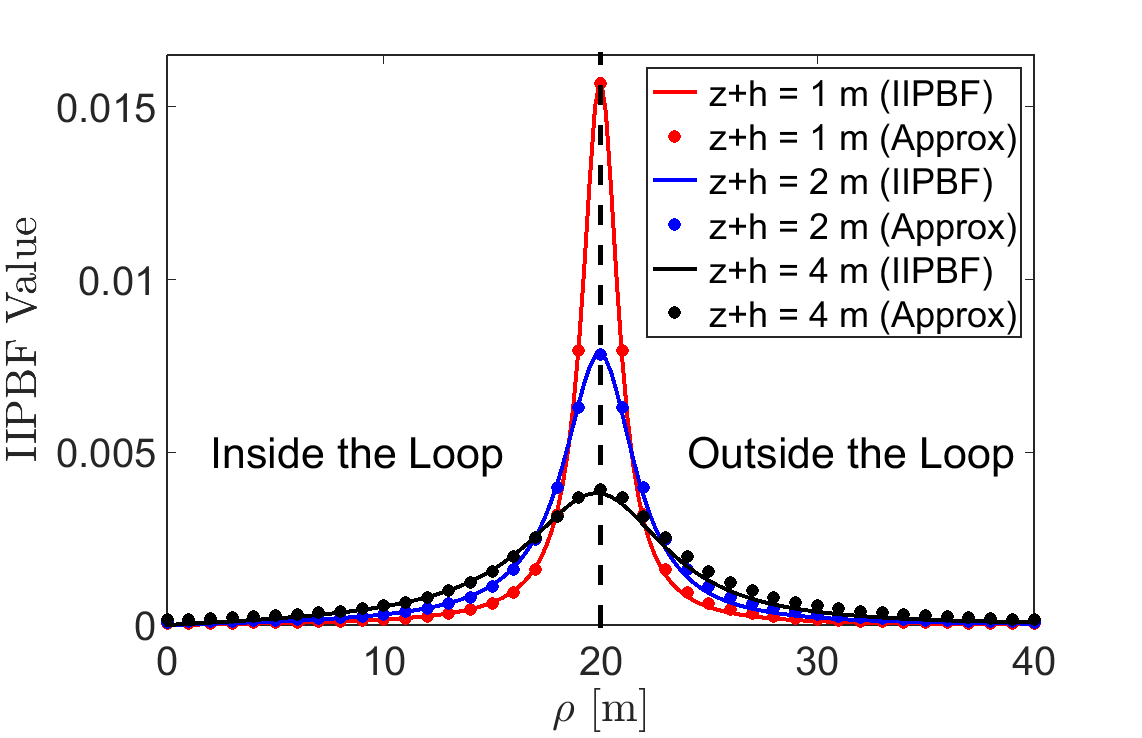
\includegraphics[width=0.50\textwidth]{DCowanVRM2017/imagesColor/figHankelJ1J1Int.png}
\vspace{15pt}
\caption{Comparison between computations of the Hankel transform using IIPBF adaptive quadrature and using the empirical expression from Eq. (\ref{eqCauchyDistr}). Comparisons are done for various values of $0 < z+h \leq a/5$, using a loop radius of $a = 20$ m.} 
\label{figHankelJ1J1Int}
\end{figure}
%---------------------------------------
%
%---------------------------------------

Now we look at the radial static response from a circular transmitter loop over a SP half-space. According to Eq. (\ref{eqBrhoMagnetostatic}), we require a solution to the integral:
\begin{equation}
\int^{\infty}_0 \lambda e^{-\lambda (z+h)} J_1(\lambda a) J_1
(\lambda \rho) d \lambda. \label{eqHankelJ1J1Int}
\end{equation}
Although analytic solutions for Eq. (\ref{eqHankelJ1J1Int}) exist \citep{Erdelyi1954}, they are too complicated to develop straightforward relationships with respect to the transmitter loop radius and observation locations. However for the special cases considered below, we can have an approximate solution.

First, let us examine the behavior of Eq. (\ref{eqHankelJ1J1Int}). For $z+h>0$, we used the IIPBF adaptive quadrature package \citep{Ratnanather2011} to evaluate the expression. Fig. \ref{figHankelJ1J1Int} shows the results for several values of $z+h$ for a loop of radius $a = 20$ m. We observed that for $0 <z+h \leq a/5$, the numerical solutions w.r.t $\rho$ behaved like a Cauchy distribution centered around $\rho = a$. As $z+h$ is decreased over the accepted range, the distribution became narrow. Therefore invoking the probability density function for a Cauchy distribution, we proposed a heuristic approximation to Eq. (\ref{eqHankelJ1J1Int}) as:
\begin{equation}
\int_0^\infty \!\!\!\! \lambda e^{-\lambda (z+h)} J_1 (\lambda a)
J_0 (\lambda \rho ) d\lambda \!\sim\! \Bigg [ \pi a \gamma \Bigg ( 1
+ \Big ( \frac{\rho - a}{\gamma } \Big )^2 \Bigg ) \Bigg ]^{-1},
\label{eqCauchyDistr}
\end{equation}
where an empirical function for $\gamma$ is given by:
\begin{equation}
\gamma = 2 (z+h) \Bigg ( \frac{2}{\pi} \Bigg )^{3/2}.
\label{eqGamma}
\end{equation}
One sees that in Fig. \ref{figHankelJ1J1Int}, the results from Eq. (\ref{eqCauchyDistr}) match well with those using IIPBF adaptive quadrature. For $z+h \rightarrow 0$, Eq. (\ref{eqHankelJ1J1Int}) approaches the Dirac delta function $\delta (x)$:
\begin{equation}
\lim_{z+h \rightarrow 0} \int^{\infty}_0 \!\!\! \lambda e^{-\lambda (z+h)} J_1(\lambda a) J_1 (\lambda \rho) d \lambda = \frac{\delta (a - \rho)}{a},
\end{equation}
which can be shown with the weighted orthogonality property of the Hankel transform \citep{Wong2008}.

By combining Eqs. (\ref{eqCauchyDistr}) and (\ref{eqBrhoMagnetostatic}), the radial static response of the SP half-space for $0 <z+h \leq a/5$ is approximated by
\begin{equation}
B_\rho^{(0)}(\rho,z) \sim -\frac{\mu_0 I}{2} \Bigg ( \frac{\Delta \chi}{2+\Delta \chi} \Bigg ) \Bigg [ \pi a \gamma \Bigg ( 1 + \Big ( \frac{\rho - a}{\gamma } \Big )^2 \Bigg ) \Bigg ]^{-1}.
\label{eqMagnetostaticGaussian}
\end{equation}
It should be noted that although Eq. (\ref{eqMagnetostaticGaussian}) provides a reasonable approximation, it cannot be used to show that $B_\rho^{(0)} (\rho \rightarrow 0,z) = 0$ exactly. This property was obtained from Eq. (\ref{eqBrhoMagnetostatic}) since $J_1 (0) = 0$.



%============================================================
%============================================================
%       NEW SECTION: VRM RESPONSE FROM A LARGE CIRCULAR LOOP
%============================================================
%============================================================

\section{VRM Response from a Large Circular Transmitter Loop}
\label{secVRMresponseFinal}
Having obtained the approximations for the after-effect function and the analytical expressions for the static fields in several cases, we now look at the VRM response with Eqs. (\ref{eqGenVRMB}) and (\ref{eqGenVRMdBdt}) over a SP half-space for $\tau_1 \ll t \ll \tau_2$.

%============================================================
%       NEW SUBSECTION: VERTICAL VRM RESPONSE
%============================================================

\subsection{Vertical VRM Response from a Large Circular Transmitter Loop}

%---------------------------------------
%       FIGURE
%---------------------------------------
\begin{figure}[!b]
    \centering
    \vspace{-10pt}
    \begin{subfigure}[b]{0.49\textwidth}
    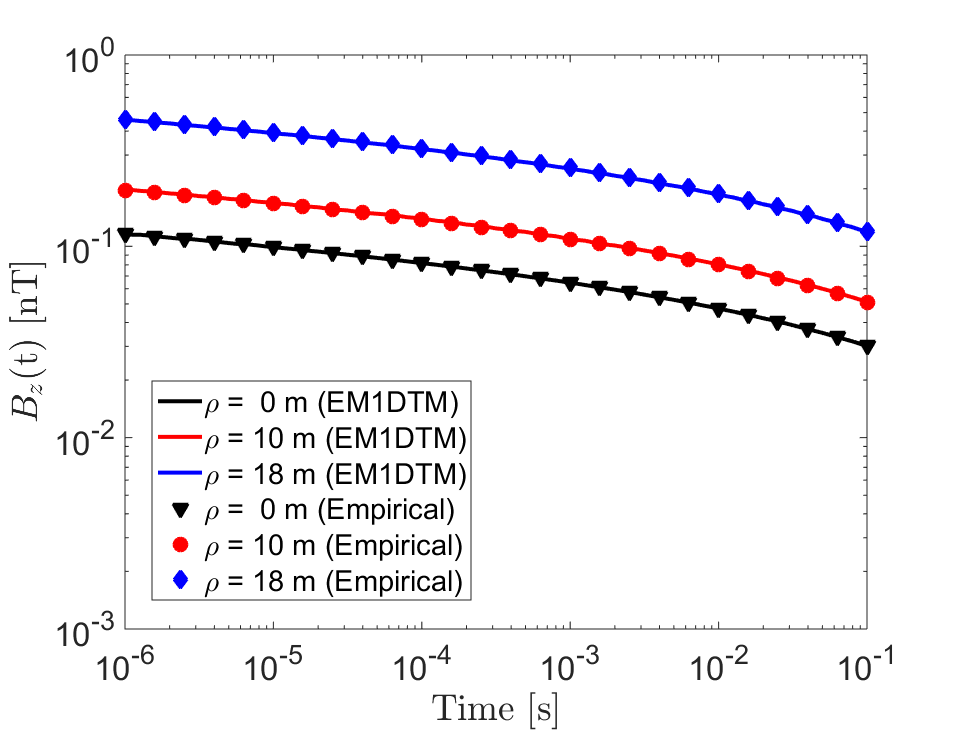
\includegraphics[width=0.4\textwidth]{DCowanVRM2017/imagesColor/figVRMrespBz.png}
    \label{figVRMrespBz}
    \end{subfigure}
    ~
    \begin{subfigure}[b]{0.49\textwidth}
    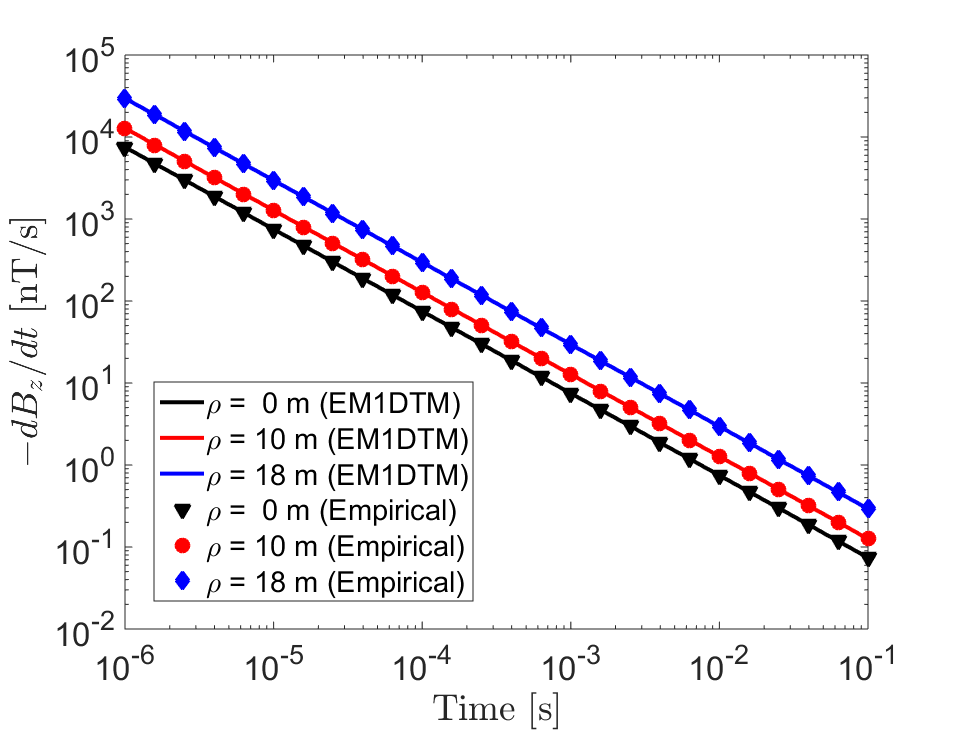
\includegraphics[width=0.4\textwidth]{DCowanVRM2017/imagesColor/figVRMrespdBzdt.png}
    \label{figVRMrespdBzdt}
    \end{subfigure}
    \caption{Vertical VRM response for a large circular loop of radius $a=20$ m on the Earth's surface, at radial distance $\rho$ from the loop's center, using properties $\Delta \chi=0.01$, $\tau_1 = 10^{-8}$ s and $\tau_2=10$ s. This plot compares expressions (\ref{eqVRMBz}) and (\ref{eqVRMdBzdt}) to values obtained using the EM1DTM code. (a) $B_z (t)$. (b) $-\partial B_z/\partial t$.}
    \label{figVRMrespZ}
\end{figure}
%----------------------------------------
%
%----------------------------------------

\subsubsection{Large Circular Loop on the Earth's Surface ($h=0$)} \label{secVertVRMresp} With expressions (\ref{eqAfterEffectB}), and (\ref{eqStaticLoopBz}), the vertical VRM response at any location $(\rho < a,z=0)$ at time $\tau_1 \ll t \ll \tau_2$ is approximated according to Eq. (\ref{eqGenVRMB})
\begin{equation}
B_z(\rho,0,t) \approx \frac{\mu_0 I}{2a} \Bigg ( \frac{\Delta
\chi}{2+\Delta \chi} \Bigg )  \Bigg [ 1 + \frac{9}{4\pi} \Bigg (
\frac{\big( \frac{\rho}{a} \big )^2}{1- \big( \frac{\rho}{a} \big
)^2} \Bigg ) \Bigg ] \bar F(t).
\label{eqVRMBz}
\end{equation}
Similarly after substitution of (\ref{eqAfterEffectdBdt}) and (\ref{eqStaticLoopBz}) into Eq. (\ref{eqGenVRMdBdt}), we have
\begin{equation} \frac{\partial B_z(\rho,0,t)}{\partial t}  \approx
\frac{\mu_0 I}{2a} \Bigg ( \frac{\Delta \chi}{2+\Delta \chi} \Bigg )
\Bigg [ 1 + \frac{9}{4\pi} \Bigg ( \frac{\big( \frac{\rho}{a} \big
)^2}{1- \big( \frac{\rho}{a} \big )^2} \Bigg ) \Bigg ] \frac{d \bar
F(t)}{dt}.
\label{eqVRMdBzdt}
\end{equation}

Both Eqs. (\ref{eqVRMBz}) and (\ref{eqVRMdBzdt}) reveal that the vertical VRM response depends upon the ratio of $\rho/a$. When an observation is made towards the center of a loop (say $\rho/a \leq 0.5$), the response tends to be small and vary minimally with respect to $\rho$. This agrees with the results obtained by others \citep{Buselli1982,Barsukov2001}. When an observation is made towards the edges of the loop, the VRM response can increase in magnitude rapidly as $\rho$ increases and $\rho/a \rightarrow 1$. Fig. \ref{figVRMrespZ} shows the variation in the VRM response when $\rho = 0 ~{\rm m}, 10 ~{\rm m}, 18 ~{\rm m}$ for a loop of radius $a=20$ m. Meanwhile, the results of Eqs. (\ref{eqVRMBz}) and (\ref{eqVRMdBzdt}) match well with those computed using the 1D numerical code-EM1DTM \cite{EM1DTM}. In practice, measurements of $B$ or $\partial B/\partial t$ are not acquired directly on the Earth's surface. Instead, data are typically collected at heights less than 1 m off the ground. Therefore for a near-surface survey with a sufficiently large loop, we should expect similar behaviour to the case above when $a \gg z$.
\\
\subsubsection{Response Along the Transmitter's Vertical Axis ($\rho = 0$)}
Using expressions (\ref{eqAfterEffectB}),  (\ref{eqGenVRMB}), and (\ref{eqStaticCoinBz}), we have the VRM response at time $\tau_1 \ll t \ll \tau_2$
\begin{equation}
\label{eqCoinB} B_z(0,z,t)  \approx \frac{\mu_0 m}{2
\pi} \Bigg ( \frac{\Delta \chi}{2 + \Delta \chi} \Bigg ) \Bigg (
\frac{1}{(z+h)^2 + a^2} \Bigg )^{3/2} \bar F(t).
\end{equation}
Similarly, using expressions (\ref{eqAfterEffectdBdt}), (\ref{eqGenVRMB}), and (\ref{eqStaticCoinBz}), we obtain:
\begin{equation}
\label{eqCoindBdt} \frac{\partial
B_z(0,z,t)}{\partial t}  \approx \frac{\mu_0 m}{2 \pi} \Bigg (
\frac{\Delta \chi}{2 + \Delta \chi} \Bigg ) \Bigg ( \frac{1}{(z+h)^2
+ a^2} \Bigg )^{3/2} \frac{d \bar F(t)}{dt}.
\end{equation}
Eqs. (\ref{eqCoinB}) and (\ref{eqCoindBdt}) show that the VRM response becomes smaller in magnitude when the size of the loop or the total elevation of $z+h$ increases. This matches analytic results and field observations made by others \citep{Lee1984,Buselli1982,Barsukov2001}. For a dipole source ($a\ll z+h$), the magnitude of the VRM response is proportional to $(z+h)^{-3}$. For $z+h=0$ and $m=\pi a^2 I$, expressions (\ref{eqCoinB}) and (\ref{eqCoindBdt}) are equivalent to expressions (\ref{eqVRMBz}) and (\ref{eqVRMdBzdt}) at $\rho=0$. The VRM response observed for a loop of radius $a=0.2$ m is shown in Fig. \ref{figVRMrespCoin} when $z + h = 1 ~{\rm m}, 2 ~{\rm m}, 4 ~{\rm m}$. Again, both the analytical and numerical results agree well.
%---------------------------------------
%       FIGURE
%---------------------------------------
\begin{figure}[!h]
    \centering
    \vspace{-10pt}
    \begin{subfigure}
    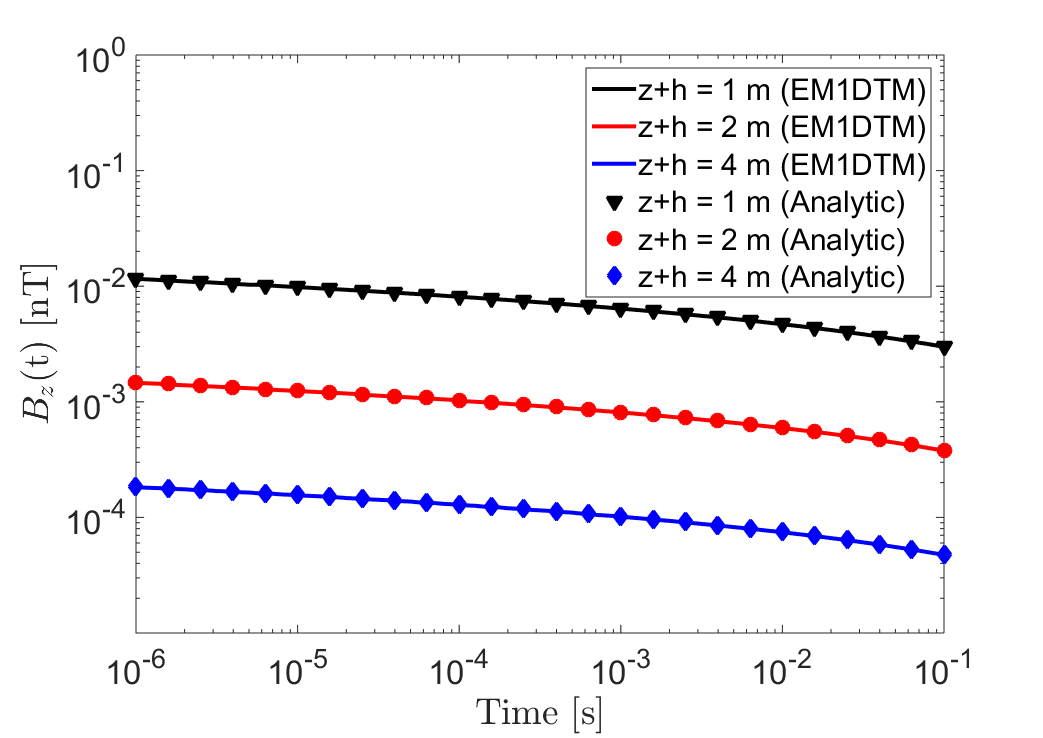
\includegraphics[width=0.40\textwidth]{DCowanVRM2017/imagesColor/figVRMrespBcoin.png}
    \label{figVRMrespBzcoin}
    \end{subfigure}\\
    \vspace{-11pt}
    \begin{subfigure}
    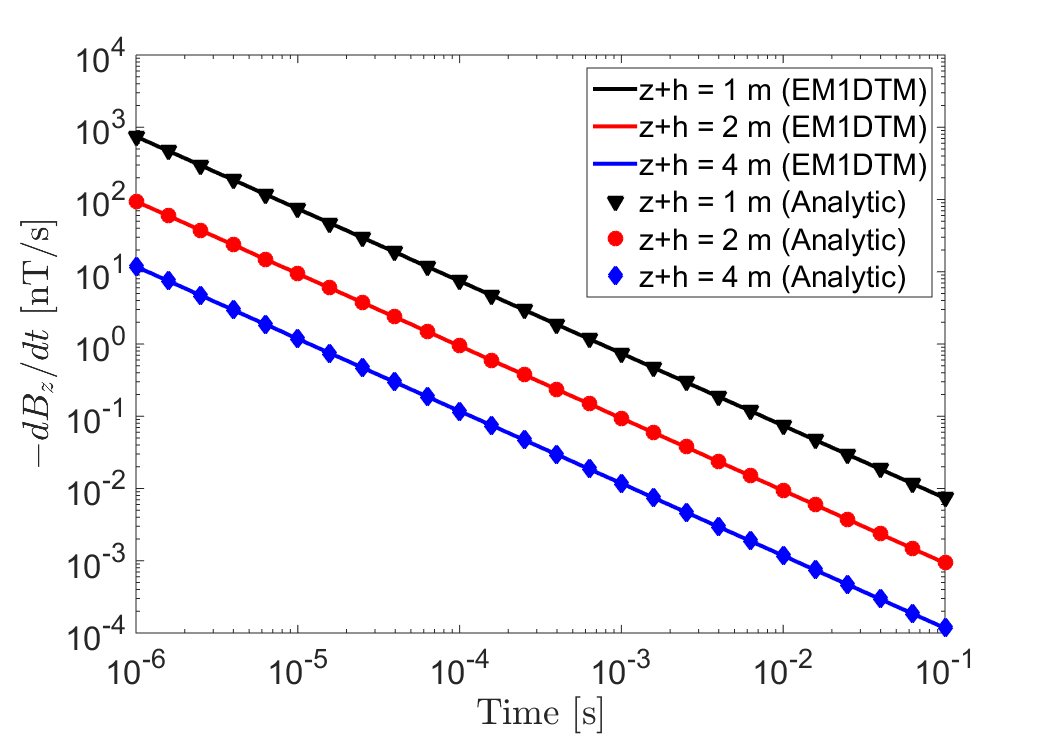
\includegraphics[width=0.40\textwidth]{DCowanVRM2017/imagesColor/figVRMrespdBdtcoin.png}
    \label{figVRMrespdBzdtcoin}
    \end{subfigure}
    \caption{Vertical VRM response along the  transmitter’s vertical axis of symmetry, using a radius of $a = 0.2$ m. Responses were predicted for several values $z+h$, using properties $\Delta \chi = 0.01$, $\tau_1 =10^{-8}$ s and $\tau_2 =10$ s. Plots compare Eqs. (\ref{eqCoinB}) and (\ref{eqCoindBdt}) to values obtained using the EM1DTM code. (a) $B_z (t)$. (b) $-\partial B_z/\partial t$.}
    \vspace{-10pt}
    \label{figVRMrespCoin}
\end{figure}
%----------------------------------------
%
%----------------------------------------

%============================================================
%       NEW SUBSECTION: RADIAL VRM RESPONSE
%============================================================

\subsection{Radial VRM Response from a Large Circular Transmitter Loop}
Using Eqs. (\ref{eqAfterEffectB}), (\ref{eqGenVRMB}), and (\ref{eqMagnetostaticGaussian}), we express the radial VRM response for $0 < z+h \leq a/5$ at time $\tau_1 \ll t \ll \tau_2$ as
\begin{equation}
B_\rho(\rho,z,t) \!\sim\! -\frac{\mu_0 I}{2}  \Bigg
( \frac{\Delta \chi}{2+\Delta \chi} \Bigg ) \! \Bigg [ \pi a \gamma
\Bigg ( 1 + \Big ( \frac{\rho - a}{\gamma } \Big )^2 \Bigg ) \Bigg
]^{-1} \!\! \bar F(t).
\label{eqGaussianB}
\end{equation}
And using expressions (\ref{eqAfterEffectdBdt}), (\ref{eqGenVRMB}) and (\ref{eqMagnetostaticGaussian}), we have
\begin{equation}
\frac{\partial B_\rho(\rho,z,t)} {\partial t}
\!\sim\! -\frac{\mu_0 I}{2} \! \Bigg ( \! \frac{\Delta
\chi}{2+\Delta \chi} \! \Bigg ) \! \Bigg [ \pi a \gamma \Bigg ( 1 +
\Big ( \frac{\rho - a}{\gamma } \Big )^2 \Bigg ) \Bigg ]^{-1} \!\!
\frac{d \bar F}{dt}.
\label{eqGaussiandBdt}
\end{equation}
Eqs. (\ref{eqGaussianB}) and (\ref{eqGaussiandBdt}) describe how the geometrical parameters can affect the response, although they are a bit more complicated than the expressions for the vertical component. Near the center of the loop, one can see that the radial component of the VRM response is small. As observations are made closer to the transmitter wire, the radial component of the VRM response increases significantly. Recall that $\gamma$ given by Eq. (\ref{eqGamma}) is a function of $z+h$. Therefore, the effect of raising the receiver off the ground can be generated by raising the transmitter off the ground. This effect was observed during field observations for various SiroTEM configurations \citep{Buselli1982}.

Figs. \ref{figVRMrespBrho} and \ref{figVRMrespdBrhodt} shows the radial VRM response for $\rho = 10 ~{\rm m}, 15 ~{\rm m}, 18 ~{\rm m}$ given a loop of radius $a=20$ m and $z+h = 1$ m. The analytical and the EM1DTM results overlap well. Similar to the vertical components, the VRM response of $B_\rho (t)$ decays in $\ln (t)$, and $\partial B_\rho / \partial t$ decays in $1/t$.
%---------- -----------------------------
%       FIGURE
%---------------------------------------
\begin{figure}[!t]
    \centering
    \begin{subfigure}
    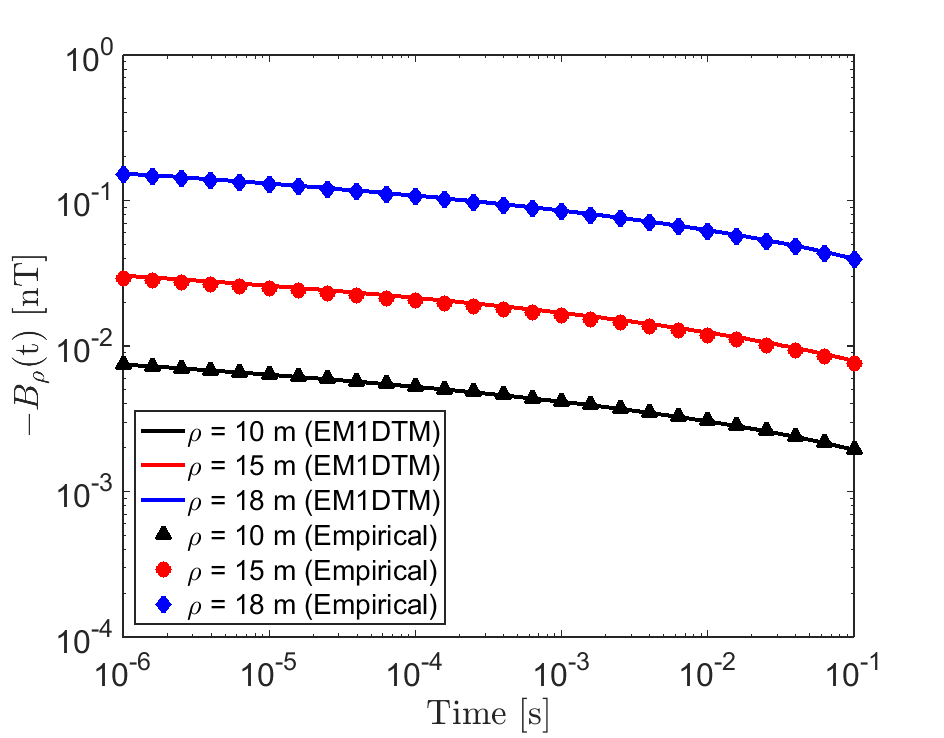
\includegraphics[width=0.4\textwidth]{DCowanVRM2017/imagesColor/figVRMrespBrho.png}
    \label{figVRMrespBrho}
    \end{subfigure}\\
    \vspace{-10pt}
    \begin{subfigure}
    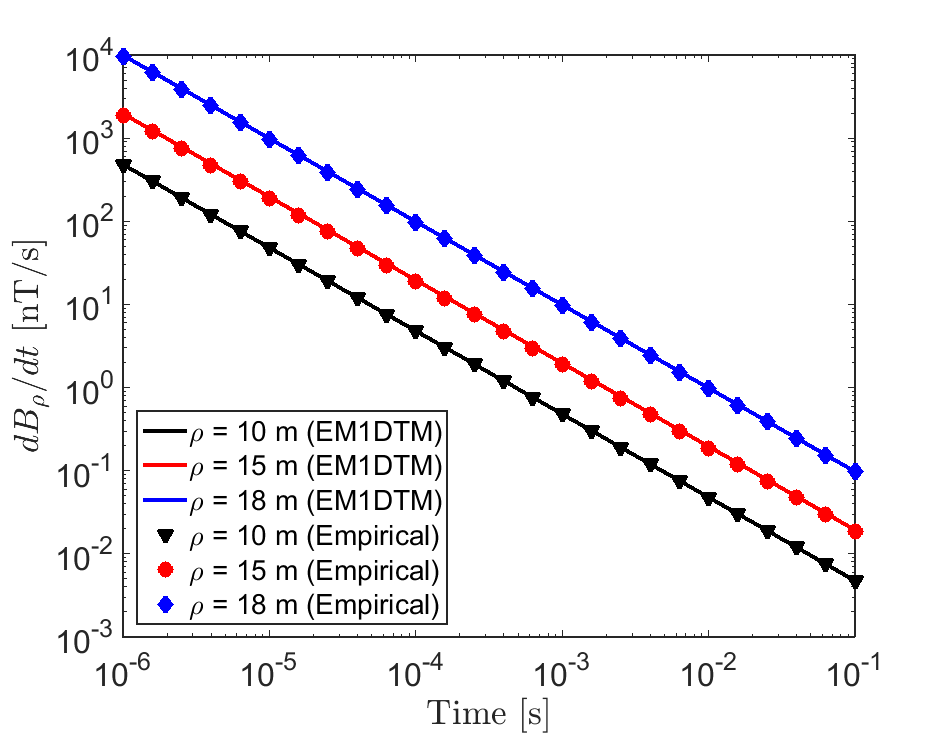
\includegraphics[width=0.4\textwidth]{DCowanVRM2017/imagesColor/figVRMrespdBrhodt.png}
    \label{figVRMrespdBrhodt}
    \end{subfigure}
    \caption{Comparison between EM1DTM and empirical functions (\ref{eqGaussianB}) and (\ref{eqGaussiandBdt}) for the radial VRM response with a loop of radius $a=20$ m. The response was predicted for $z+h =20$ m using physical properties $\Delta \chi = 0.01$, $\tau_1 =10^{-8}$ s and $\tau_2 =10$ s. (a) $-B_\rho (t)$. (b) $dB_\rho /dt$.}
\label{figVRMrespRadial}
\vspace{-10pt}
\end{figure}
%----------------------------------------
%
%----------------------------------------

%======================================================
%======================================================
%               NEW SECTION: INDUCTIVE VS VRM RESPONSE
%======================================================
%======================================================

\section{Response over a Conductive and Magnetically Viscous Half-Space}
\label{secEMversusVRM}

The magnetic susceptibilities of lateritic soils are generally low ($\chi < 0.01$) \citep{vanDam2004,vanDam2005,Druyts2009}; as such, the magnetic properties of lateritic soils do not have a significant impact on the inductive response. Some studies showed that effects of conductivity may be neglected when considering the soil's VRM response \citep{Billings2003,Druyts2009,Das2006}. Some have suggested that the inductive and VRM responses from lateritic soils are approximately separable \citep{Pasion2007,Buselli1982,Das2006}. In this section, we will test this assumption using the 1D numerical modeling code (EM1DTM) \citep{EM1DTM} over a half-space model. Given that the inductive and VRM responses are separable, we present the critical time analysis by comparing the vertical inductive and VRM responses with respect to the loop's radius and observation distances.



%============================================================
%       NEW SUBSECTION: SEPARABILITY OF THE VRM RESPONSE
%============================================================


\subsection{Separation of Inducitve and VRM responses}
\label{secSeparable} Consider a conductive and magnetically viscous half-space with $\sigma = 0.01$ S/m, $\chi_\infty = 0$, $\Delta \chi = 0.001$, $\tau_1 = 10^{-8}$ s and $\tau_2 = 10$ s. Fig. \ref{figVRMrespZadd} shows the inductive, the VRM , and the total transient responses computed by EM1DTM for a loop of radius $a=20$ m on the surface. One sees that for the vertical and radial components after sufficient time, the observed response becomes dominated by the VRM response; whereas the early times appear to be dominated by the inductive response. The numerical results verify that the total response for a conductive and magnetically viscous Earth can be well approximated as the sum of the individual inductive and VRM responses and support the observations made by \citep{vanDam2004, vanDam2005,Druyts2009, Billings2003,Das2006,Pasion2007,Buselli1982}. Overall, we found that for sufficiently small DC susceptibilities ($\chi_\infty + \Delta \chi < 0.01$), inductive and VRM responses could be predicted independently. For larger values of $\chi_\infty + \Delta \chi$, magnetic properties can affect the inductive response. On the other hand, the VRM response was insensitive to changes to the half-space conductivity. Bear in mind that the value of $\chi_\infty$ has no effect on the VRM response as the contribution made by instantaneous magnetization during the off-time is zero.

%---------------------------------------
%       FIGURE
%---------------------------------------
\begin{figure}[!t]
    \centering
    \vspace{-10pt}
    \begin{subfigure}
    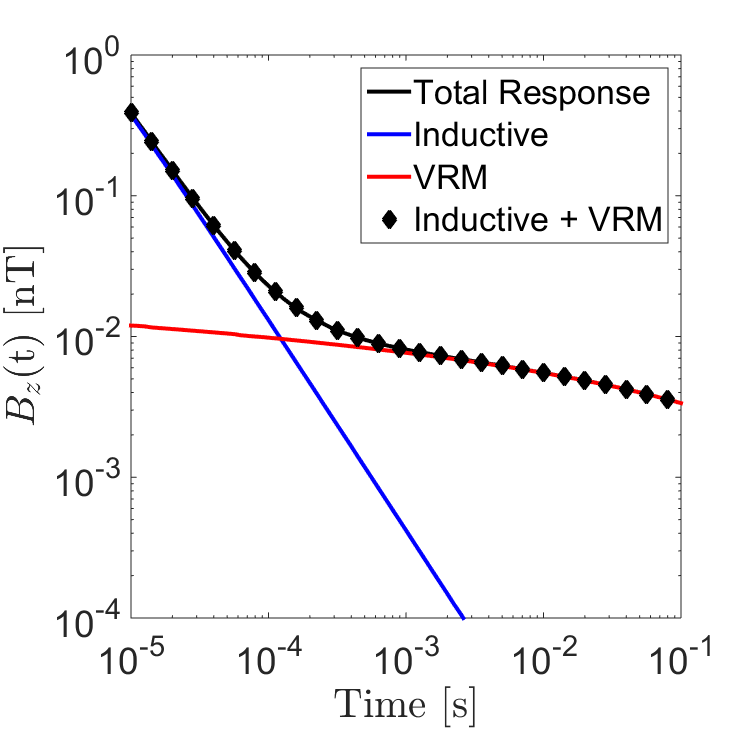
\includegraphics[width=0.35\textwidth]{DCowanVRM2017/imagesColor/figBzAdditive.png}
    \label{figBzAdditive}
    \end{subfigure}
    \begin{subfigure}
    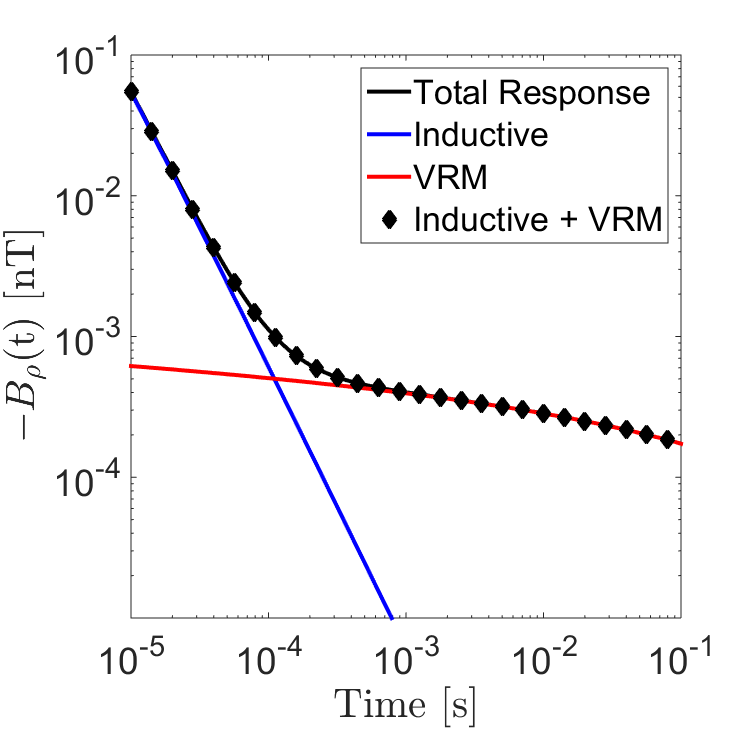
\includegraphics[width=0.35\textwidth]{DCowanVRM2017/imagesColor/figBrhoAdditive.png}
    \label{figBrhoAdditive}
    \end{subfigure}\\
    \begin{subfigure}
    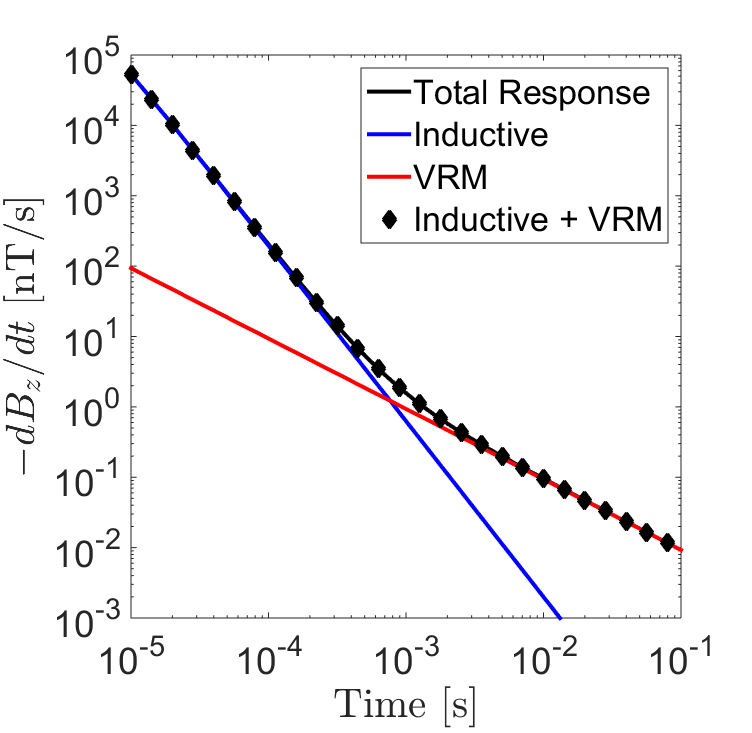
\includegraphics[width=0.35\textwidth]{DCowanVRM2017/imagesColor/figdBzdtAdditive.png}
    \label{figdBzdtAdditive}
    \end{subfigure}
    \begin{subfigure}
    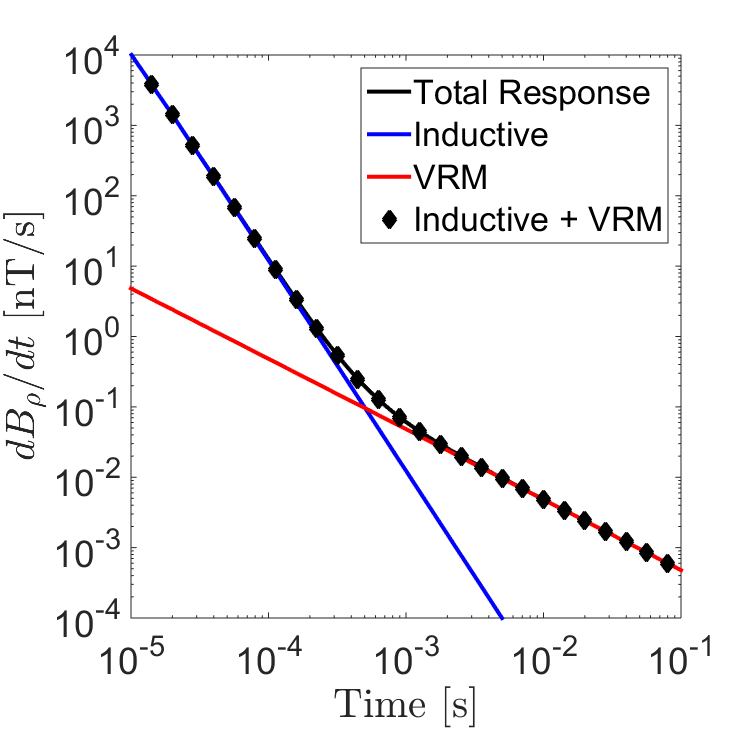
\includegraphics[width=0.35\textwidth]{DCowanVRM2017/imagesColor/figdBrhodtAdditive.png}
    \label{figdBrhodtAdditive}
    \end{subfigure}
    \caption{Additivity of the inductive and VRM responses for a loop of radius $a=20$ m at location ($\rho,z$) = (10 m, 1 m). The half-space was given physical properties: $\sigma = 0.01$ S/m, $\chi_{\infty} = 0$, $\Delta \chi = 0.001$, $\tau_1 = 10^{-8}$ s and $\tau_2 = 10$ s. (a) $B_z (t)$. (b) $-B_\rho (t)$. (c) $-\partial B_z/\partial t$. (d) $\partial B_\rho /\partial t$.}
    \label{figVRMrespZadd}
\end{figure}
%----------------------------------------
%
%----------------------------------------

%============================================================
%       NEW SUBSECTION: INDUCTIVE VS VRM
%============================================================

\subsection{Estimating the Cross-Over Time of VRM Responses}
\label{secIndVsVRM}
\cite{Nabighian1979} showed that for a step-off excitation, to first-order, the quasi-static inductive response within a large circular transmitter loop on the surface of a conductive half-space would approach the following expression asymptotically after sufficient time:
\begin{equation}
\label{eqKaufmanB}
B_z(t) \approx \frac{I \sigma^{3/2} \mu_0^{5/2} a^2}{30 \sqrt{\pi}} t^{-3/2}
\end{equation}
and that:
\begin{equation}
\label{eqKaufmandBdt}
\frac{\partial B_z}{\partial t} \approx -\frac{ I \sigma^{3/2} \mu_0^{5/2} a^2}{20 \sqrt{\pi}} t^{-5/2}
\end{equation}
where $a$ is the loop's radius, $\sigma$ is the Earth's conductivity and $\mu_0$ is the permeability of free space. Note that the inductive response and its derivative decay according to $t^{-3/2}$ and $t^{-5/2}$ respectively. Futhermore, the strength of the inductive response is proportional to $a^2$.

As the inductive and VRM responses can be predicted independently, we want to inspect how both responses change over time. Refer to Fig. \ref{figVRMrespZadd}. We observe that the decay rate of the total response starts to change roughly at a time when the inductive curve intersects with the VRM curve. Thus by setting up the ratio between the vertical inductive response $B_z^{(IND)}$ and the vertical VRM response $B_z^{(VRM)}$ with (\ref{eqAfterEffectB}), (\ref{eqVRMBz}) and (\ref{eqKaufmanB})
\begin{align}
R_B &= \frac{B_z^{(IND)}}{B_z^{(VRM)} } \nonumber \\
&\approx \! \frac{\ln(\tau_2/\tau_1)}{15 \, Q(\rho /a) \sqrt{\pi}}
\! \Bigg ( \frac{2+\Delta \chi}{\Delta \chi} \Bigg ) \! \Bigg (
\frac{t^{-3/2}}{-\gamma - \ln(t/ \tau_2)} \Bigg ) \! (\mu_0
\sigma)^{3/2} a^3 \label{eqRB}
\end{align}
and for the derivative with (\ref{eqAfterEffectdBdt}), (\ref{eqVRMdBzdt}) and (\ref{eqKaufmandBdt})
\begin{align}
R_{dB/dt} &= \frac{\partial B_z/ \partial t^{(IND)}}{\partial B_z/\partial t^{(VRM)} }  \nonumber \\
&\approx \frac{\ln(\tau_2/\tau_1)}{10 \, Q (\rho /a) \sqrt{\pi}}
\Bigg ( \frac{2+\Delta \chi}{\Delta \chi} \Bigg ) (\mu_0
\sigma)^{3/2} a^3 t^{-3/2},
\label{eqRdBdt}
\end{align}
we can estimate the time at which magnetic viscosity begins to dominate the vertical observed response. Such times are called the cross-over time. Let $t_{\alpha}$ denote the cross-over time for $B_z$, which solves $R_B=1$ in Eq. (\ref{eqRB}) . And let $t_{\beta}$ denote  the cross-over time for $\partial B_z/\partial t$, which solves $R_{dB/dt}=1$ in Eq. (\ref{eqRdBdt}). For $\partial B_z/\partial t$, the cross-over time $t_\beta$ is straightforward:
\begin{equation}
\label{eqtbeta} t_{\beta} \approx \Bigg [
\frac{\ln(\tau_2/\tau_1)}{10 \, Q (\rho /a) \sqrt{\pi}} \Bigg  (
\frac{2+\Delta \chi}{\Delta \chi} \Bigg ) \Bigg ]^{2/3} \mu_0 \sigma a^2
\end{equation}
%----------------------------------------
%       FIGURE
%----------------------------------------
\begin{figure}[!t]
\centering
\vspace{-10pt}
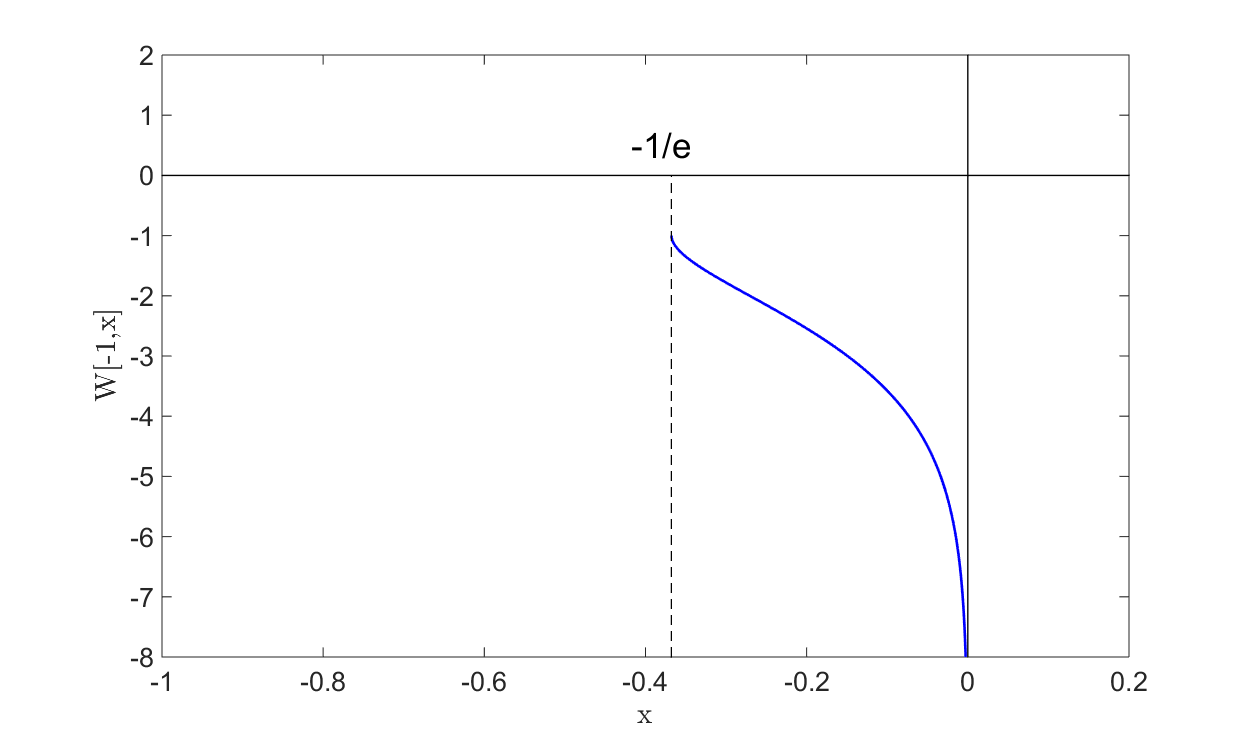
\includegraphics[width=0.48\textwidth]{DCowanVRM2017/imagesColor/figW.png}
\caption{Lower branch of the Lambert W function $W[-1,x]$ for values $-1/e \leq x \leq 0$.}
\label{figW}
\end{figure}
%----------------------------------------
Eq. (\ref{eqtbeta}) states that by increasing the radius of a transmitter loop,  the expected time $t_\beta$ at which $\partial B_z/\partial t$ becomes dominated by the VRM response is pushed to a later time. At the center of any loop, $Q=1$ and $t_{\beta} \propto \sigma a^2$. Because $t_\beta \propto Q^{-2/3}$, as an observation moves towards the edge of the loop, we expect $t_\beta$ to decrease and thus the VRM response starts to dominate earlier.

For $B_z(t)$, the VRM response begins to dominate at time:
\begin{equation}
\label{eqtalpha}
t_\alpha \approx  t_\beta \Bigg ( - W \Bigg [ - \! 1, - \Big ( \frac{t_\beta}{\tau_2} e^\gamma \Big )^{3/2} \Bigg ] \Bigg )^{-2/3} \leq t_\beta
\end{equation}
where $W[-1,x]$ is the lower branch of the  Lambert W function \cite{Corless1996}, $\gamma = 0.5772$ is the Euler constant, and $t_\beta$ is given in (\ref{eqtbeta}). $W[-1,x]$ for values $-1/e \leq x \leq 0$ is shown in Fig. (\ref{figW}). Its derivation can be found in the Appendix.

Eq. (\ref{eqtalpha}) shows that $t_\alpha$ is a monotonic increasing function with respect to $t_\beta$. Although the dependence of $t_\alpha$ on $a$ and $Q(\rho/a)$ is not straightforwardly represented in Eq. (\ref{eqtalpha}), we can qualitatively infer that TEM instruments which measure $B_z(t)$ are much more affected by the VRM response than instruments which measure $\partial B_z/\partial t$. It can be shown that $t_\alpha \ll t_\beta$ for $t_\beta \ll \tau_2 e^\gamma$.
%----------------------------------------
%
%----------------------------------------
\begin{figure}[!b]
    \centering
    \vspace{-15pt}
    \begin{subfigure}
    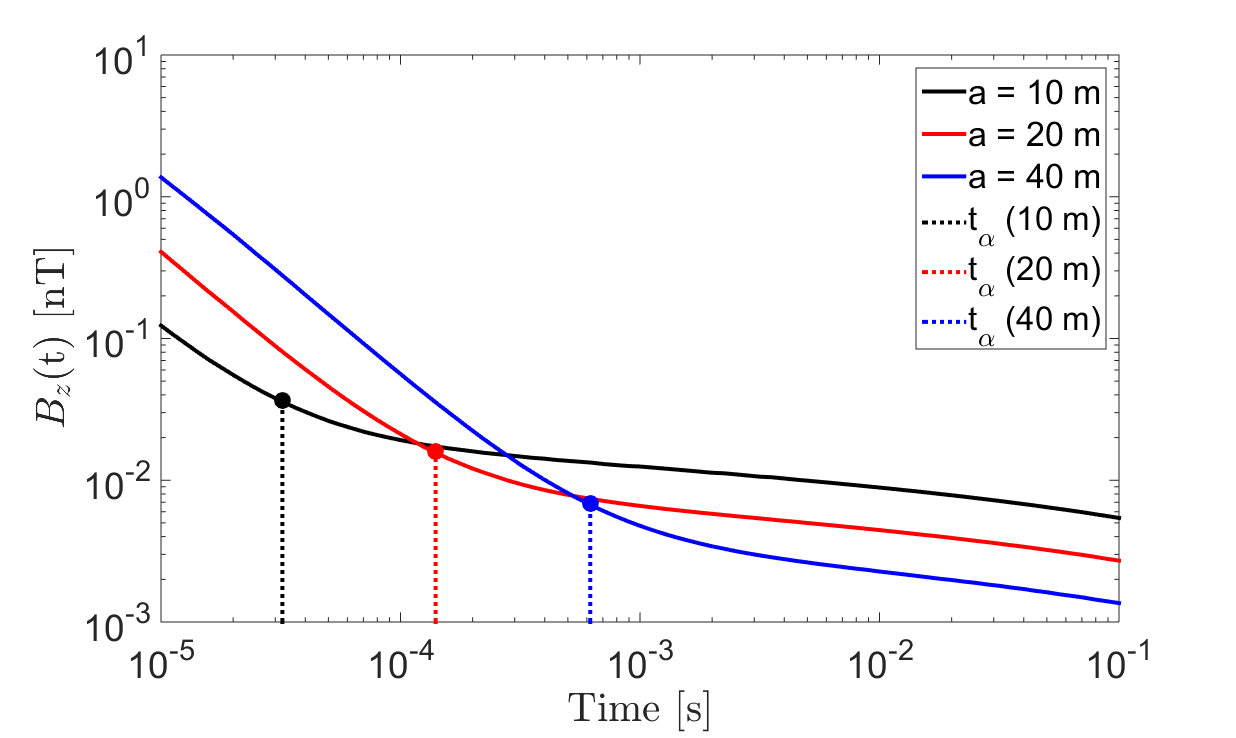
\includegraphics[width=0.45\textwidth]{DCowanVRM2017/imagesColor/figEMandVRMrespBzCenterLoops.png}
    \label{figRespBzLoops}
    \end{subfigure}\\
    \vspace{-10pt}
    \begin{subfigure}
    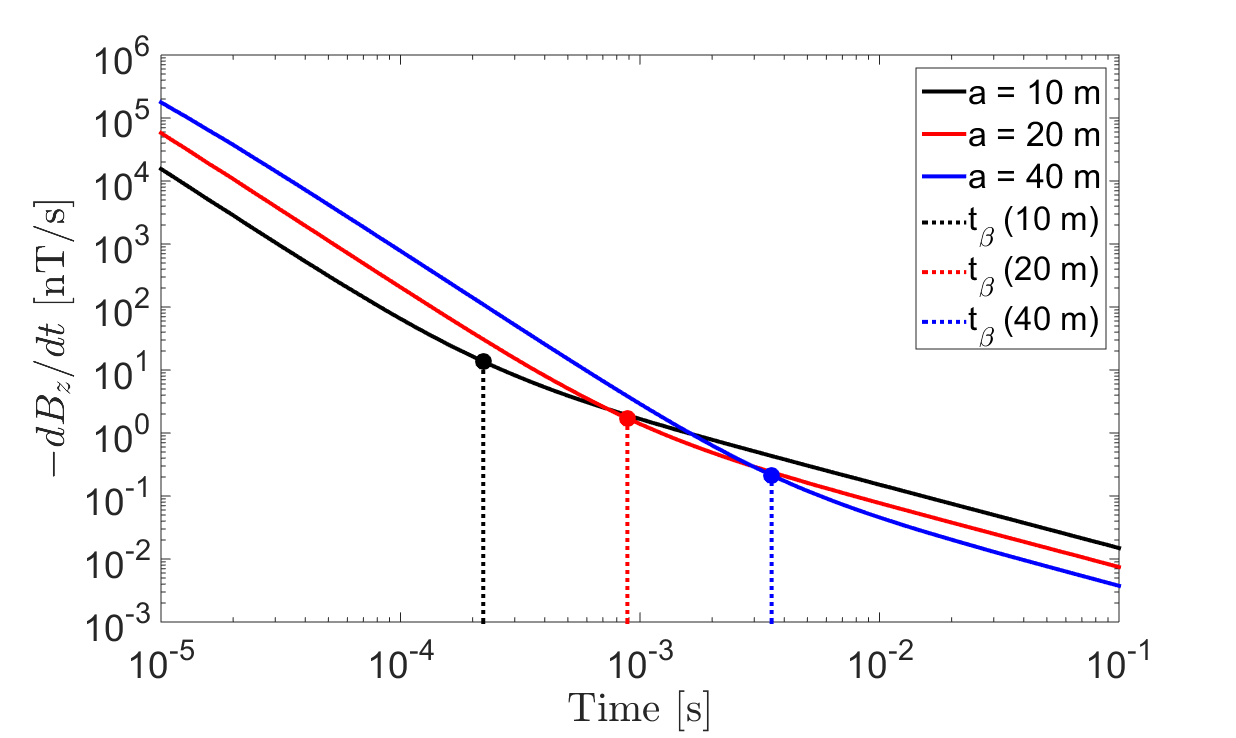
\includegraphics[width=0.45\textwidth]{DCowanVRM2017/imagesColor/figEMandVRMrespdBzdtCenterLoops.png}
    \label{figRespdBzdtLoops}
    \end{subfigure}
    \caption{Vertical transient response at the center of a set of transmitter loops with varying radii, located on the Earth's surface. EM1DTM was used to predict the responses for a half-space with physical properties: $\sigma=10^{-2}$ S/m, $\Delta \chi=0.001$, $\tau_1=10^{-8}$ s and $\tau_2=10$ s. (a) $B_z (t)$. (b) $-\partial B_z/\partial t$.}
    \label{figEMandVRMrespLoops}
\end{figure}
%----------------------------------------
%
%----------------------------------------
Fig. \ref{figEMandVRMrespLoops} shows the vertical transient responses calculated using the EM1DTM at the center of a transmitter loop when the radius $a = 10$ m, 20 m, 40 m. $t_{\alpha}$ and its corresponding value $B_z(t)$ were calculated using Eqs. (\ref{eqAfterEffectB}), (\ref{eqVRMBz}), (\ref{eqKaufmanB}) and (\ref{eqtalpha}); $t_{\beta}$ and its corresponding value $dB_z/dt$ were calculated using Eqs. (\ref{eqAfterEffectdBdt}), (\ref{eqVRMdBzdt}), (\ref{eqKaufmandBdt}) and (\ref{eqtbeta}). It confirms that $t_\alpha$ and $t_\beta$ increase with respect to $a$, and that $t_\alpha \leq t_\beta$. 

Consider the vertical transient responses in Fig. \ref{figEMandVRMrespOffAxis} at various radial locations $\rho$ for a transmitter loop with radius $a=20$ m. $t_{\alpha}$ and its corresponding value $B_z(t)$ were calculated using Eqs.(\ref{eqAfterEffectB}), (\ref{eqVRMBz}), (\ref{eqKaufmanB}) and (\ref{eqtalpha}); $t_{\beta}$ and its corresponding value $\partial B_z/\partial t$ were calculated using Eqs. (\ref{eqAfterEffectdBdt}), (\ref{eqVRMdBzdt}), (\ref{eqKaufmandBdt}) and (\ref{eqtbeta}). Similarly, we observe that $t_\alpha$ and $t_\beta$ decrease with respect to $\rho$, and that $t_\alpha \leq t_\beta$. Recall that $Q$ in Eq. (\ref{eqElliptic}) increases as $\rho \rightarrow a$. Thus when observations are made closer to the transmitter loop, the VRM response will not only increase but will also dominate the total observed transient response at earlier times. This is consistent with the observation that magnetic viscosity is known to be most problematic near the transmitter wire \cite{Buselli1982,Lee1984,Barsukov2001}.

%----------------------------------------
%
%----------------------------------------
\begin{figure}[!t]
    \centering
    \begin{subfigure}
    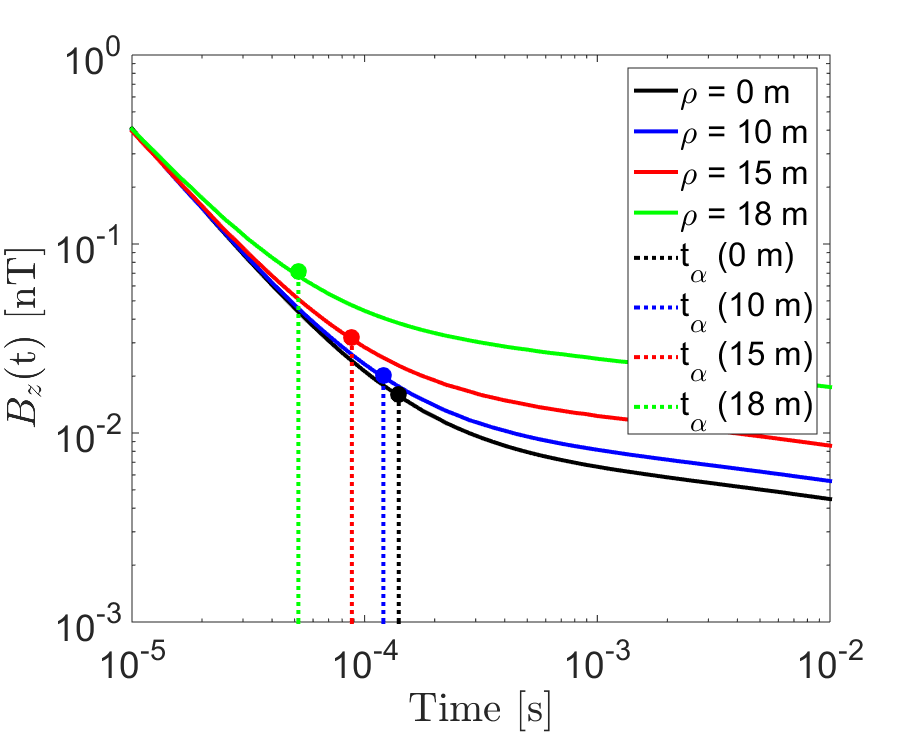
\includegraphics[width=0.45\textwidth]{DCowanVRM2017/imagesColor/figEMandVRMrespBzOffAxis.png}
    \label{figEMandVRMoffaxisBz}
    \end{subfigure}\\
    \vspace{-10pt}
    \begin{subfigure}
    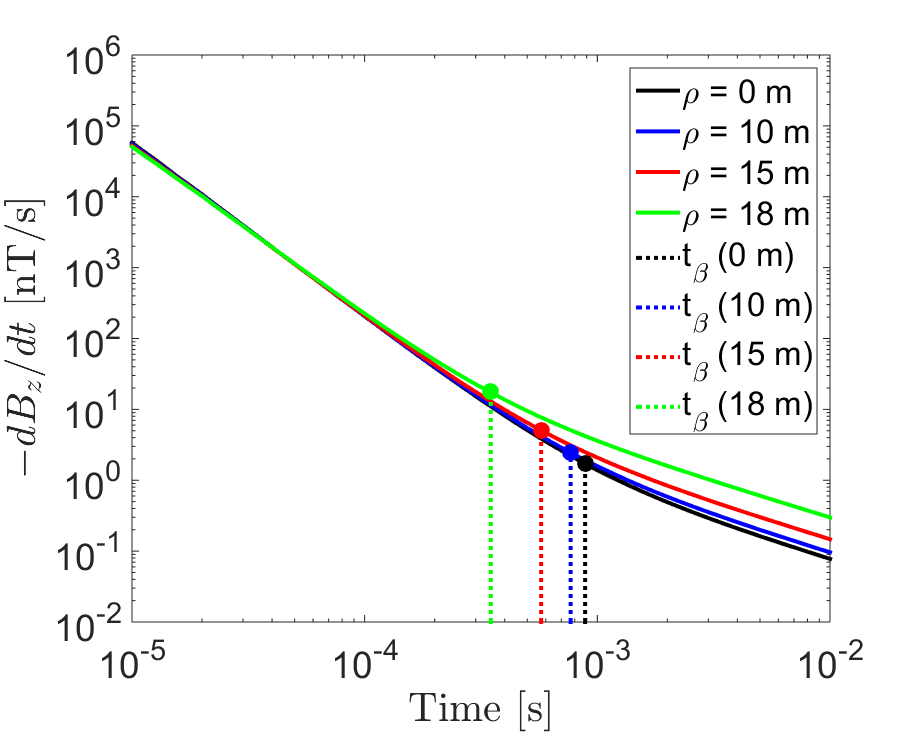
\includegraphics[width=0.45\textwidth]{DCowanVRM2017/imagesColor/figEMandVRMrespdBzdtOffAxis.png}
    \label{figEMandVRMoffaxisdBzdt}
    \end{subfigure}
    \caption{Vertical transient response at off-axis locations $\rho$, for a loop of radius $a=20$ m, located on the Earth's surface. EM1DTM was used to predict the responses for a half-space with physical properties: $\sigma=10^{-2}$ S/m, $\Delta \chi=0.001$, $\tau_1=10^{-8}$ s and $\tau_2=10$ s. (a) $B_z (t)$. (b) $-\partial B_z/\partial t$.}
    \label{figEMandVRMrespOffAxis}
\end{figure}
%----------------------------------------
%
%----------------------------------------

Figs. \ref{figEMandVRMrespLoops} and \ref{figEMandVRMrespOffAxis} demonstrate how Eqs. (\ref{eqtbeta}) and (\ref{eqtalpha}) can be used to estimate the cross-over times (dashed lines) at which $B_z (t)$ and $\partial B_z /\partial t$ within the loop become dominated by the VRM response.  The projection of $t_\alpha$ and $t_\beta$ on the corresponding total response curve will appear earlier than the point of maximum curvature on each log-log plot (also see Fig. \ref{figVRMrespZadd}). Provided that a-priori information is supplied regarding the Earth's physical properties, Eqs. (\ref{eqRB}) through (\ref{eqtalpha}) can provide some survey guides in practice. For example, Eqs. (\ref{eqRB}) and (\ref{eqRdBdt}) can be used to help adjust a loop size that renders the VRM response negligible over a specified time range. With an estimated cross-over time, one can properly remove the VRM effects during the late-time response.





%======================================================
%======================================================
%               NEW SECTION: CONCLUSION
%======================================================
%======================================================

\section{Conclusion}
In this paper, we have presented the analytical formulae for the transient VRM response generated by a large circular loop over a magnetically viscous half-space for a step-off excitation. Assuming that the soil's magnetic viscosity is represented by a collection of non-interacting SP grains \citep{Neel1949} and that magnetic fields are governed by the magnetostatic law, we can express the VRM response and its derivatives as the product of a static field and an after-effect time function. We approximated the true after-effect function of the half-space by using a log-uniform distribution of time-relaxation constants to characterize the magnetic viscosity. As for the static fields, we derived the associated expressions by simplifying and approximating Hankel integrals for the vertical and radial field components. Analytic expressions were verified with the 1D forward modelling code \citep{EM1DTM}. Both analytical and numerical results showed excellent agreement for sufficiently small magnetic susceptibilities.

Our analytic expressions explicitly reveal how the VRM response depends upon geometric survey properties such as the transmitter loop's size and the observation location within the loop. For vertical VRM responses measured near the surface, the ratio of $\rho/a$ plays a major role in controlling the magnitude. When $\rho/a \rightarrow 1$, i.e., an observation is made towards the edge of the loop, VRM responses can increase significantly. Equivalently, strong VRM responses are expected for a smaller transmitter loops. For measurements along the axis of the loop, the vertical VRM response  can be diminished by either increasing the sensor height or increasing the size of the loop. For radial VRM responses, our empirical approximation predicts that it is small near the center of the loop. As observations are made closer to the transmitter wire, the increased strength of radial VRM response can be damped by increasing the sensor height. Characteristics of the VRM response uncovered in the analytical expressions are consistent with other field observations and numerical modeling results \citep{Buselli1982, Barsukov2001, Billings2003, Kozhevnikov2007,Pasion2007, Zadorozhnaya2012}.

Furthermore, we have suggested an estimate of the cross-over time from which the response might be divided into earlyinductive and late VRM stages. Increasing the size of a loop can push the cross-over time to a later time. On the other hand, a near loop-edge observation tends to have an early cross-over time. Also, we found that the VRM response impacts on the magnetic flux density $B(t)$ at much earlier times than on its time derivative $dB/dt$. Therefore in regions where lateritic soils are prominent, it may not be recommended to use TEM systems that only measure the magnetic flux density; which are potentially contaminated by the VRM signal across a larger number of time channels.

Overall, our analytical expressions can serve as a convenient design code for choosing an appropriate loop size and selecting an optimal range of observation times. This may prove beneficial when attempting to reduce the VRM response or pinpoint a certain time window where the VRM response can be properly removed.



%======================================================
%======================================================
%               NEW SECTION: ACKNOWLEDGEMENTS
%======================================================
%======================================================

% \begin{appendix}

% \setcounter{equation}{0}
% \numberwithin{equation}{section}

% We wish to solve expression (\ref{eqRB}) for $R_B=1$ to obtain
% expression (\ref{eqtalpha}).  This is equivalent to solving an
% expression of the form:
% \begin{equation}
% \label{eqLnPoly} A t^{-3/2} + \ln t \approx -\gamma + \ln \tau_2,
% \end{equation}
% where
% \begin{equation}
% \label{eqA} A = \frac{\ln(\tau_2/\tau_1)}{15 \, Q(\rho /a)
% \sqrt{\pi}} \! \Bigg ( \frac{2+\Delta \chi}{\Delta \chi} \Bigg )
% (\mu_0 \sigma)^{3/2} a^3.
% \end{equation}
% Changing the variable $u=t^{-3/2}$, and with some algebra, we can
% rewrite Eq. (\ref{eqLnPoly}) as
% \begin{equation}
% \label{eqVarChange} - \frac{3}{2} A u e^{- \frac{3}{2} A u} \approx
% - \frac{3}{2} A e^{\frac{3}{2} (\gamma - \ln \tau_2)}.
% \end{equation}
% Solutions to an expression of the form $x e^x = C$ are defined as
% branches of the  Lambert W function $W[n,C]$, where $n$ are integer
% values \cite{Corless1996}. Therefore, the solutions $u_n$ to Eq.
% (\ref{eqVarChange}) are
% \begin{equation}
% u_n \approx - \frac{2}{3A} W \Big [ n, - \frac{3}{2} A
% e^{\frac{3}{2}(\gamma - \ln \tau_2)} \Big ]
% \end{equation}
% We can use Eqs. (\ref{eqtbeta}) and (\ref{eqA}) to
% show $A = \frac{2}{3} t_\beta^{3/2}$. By replacing $u_n =
% t_n^{-3/2}$:
% \begin{align}
% &t_n^{-3/2} \approx - t_\beta^{-3/2} W \Big [ n, - t_\beta^{3/2} e^{\frac{3}{2}(\gamma - \ln \tau_2)} \Big ] \nonumber \\
% \label{eqWsol}
% \implies \; \; &t_n \approx t_\beta \Bigg ( - W \Bigg [ n, - \Big ( \frac{t_\beta}{\tau_2} e^\gamma \Big )^{3/2} \Bigg ] \Bigg )^{-2/3}
% \end{align}

% Real-valued solutions $W[n,x]$ only exist for
% $n=-1,0$ \cite{Corless1996}.  Additionally, for $t_n$ to occur after
% the primary field has been removed ($t_n \geq 0$), $W [n,x]$
% requires $-1/e \leq x \leq 0$. Thus, by Eq. (\ref{eqWsol}):
% \begin{align}
% & -1/e \leq - \Big ( \frac{t_\beta}{\tau_2}e^\gamma \Big )^{3/2} \leq 0 \nonumber \\
% \label{eqWcond}
% \implies & e^{-\frac{2}{3}-\gamma} \approx 0.288267 \geq \frac{t_\beta}{\tau_2} \geq 0
% \end{align}

% Recall that our choice in after-effect function
% (\ref{eqAfterEffectB})  is only valid for $\tau_1 \ll t \ll \tau_2$.
% Therefore, the condition defined in expression (\ref{eqWcond}) is
% reasonable under the assumption that $t_\beta \ll \tau_2$. We
% evaluated Eq. (\ref{eqWsol}) for $n=0$ and noticed the solutions were
% $t_0 \not \ll \tau_2$. This violates our conditions for the
% after-effect function and is therefore not a valid solution. On the other hand, solutions of Eq.
% (\ref{eqWsol}) for $n=-1$ did not violate
% conditions for the after-effect function. The solutions
% obtained using $W[-1,x]$ consistently showed $t_\alpha \leq
% t_\beta$. As a result, the time $t_\alpha$ which solves $R_B=1$ in
% expression (\ref{eqRB}) is given by:
% %\setcounter{equation}{50}
% \begin{equation} t_\alpha \approx  t_\beta \Bigg ( -
% W \Bigg [ - \! 1, - \Big  ( \frac{t_\beta}{\tau_2} e^\gamma \Big
% )^{3/2} \Bigg ] \Bigg )^{-2/3} \leq t_\beta \tag{47}
% \end{equation}
% \end{appendix}


%======================================================
%======================================================
%               NEW SECTION: ACKNOWLEDGEMENTS
%======================================================
%======================================================

%\section*{Acknowledgments}
%
%I would like to thank Dr. Lin Ping Song and Dr. Doug Oldenburg for the mentorship I have received during my studies at the University of British Columbia.





%======================================================
%======================================================
%               NEW SECTION: REFERENCES
%======================================================
%======================================================

%\begin{thebibliography}{100}
%
%% (1)
%\bibitem{Buselli1982}
%G. Buselli, "The effect of near-surface superparamagnetic material on electromagnetic measurements," \emph{Geophysics}, vol. 47, no. 9, pp. 1315-1324, Sep 1982.
%
%% (2)
%\bibitem{Barsukov2001}
%P.~O. Barsukov, E.~B. Fainberg, "Superparamagnetic Effect Over Gold and Nickel Deposits," \emph{European Journal of Environmental and Engineering Geophysics}, vol. 6, pp. 61-72, 2001.
%
%% (3)
%\bibitem{Billings2003}
%S.~D. Billings, L.~R. Pasion, D.~W. Oldenburg and J. Foley, "The influence of magnetic viscosity on electromagnetic sensors," \emph{Proceedings of EUDEM-SCOT2, International Conference on Requirements and Technologies for the Detection, Removal and Neutralization of Landmines and UXO}, 2003.
%
%% (4)
%\bibitem{Pasion2007}
%L.~R. Pasion, "Inversion of Time Domain Electromagnetic Data for the Detection of Unexploded Ordnance," Ph.D. dissertation, Univ. of British Columbia, Geophysics Dept., Vancouver, 2007.
%
%% (5)
%\bibitem{Zadorozhnaya2012}
%V.~Y. Zadorozhnaya, N.~O. Kozhevnikov, P. Nyabeze, "Superparamagnetic Effect, Effect Provided by 'Red Soil' in Southern Africa," in \emph{21\textsuperscript{st} EM Induction Workshop}, Darwin, July 25-31, 2012.
%
%% (6)
%\bibitem{Dabas1992}
%M. Dabas, A. Jolivet, A. Tabbagh, "Magnetic Susceptibility and Viscosity of Soils in a Weak Time Varying Field," \emph{Geophys. J. Int.}, vol. 108, pp. 101-109, 1992.
%
%% (7)
%\bibitem{Neel1949}
%L. N\'{e}el, "Th\'{e}orie du trainage magne\'{e}tique des ferromagnetiques en grains fins avec application au terres cuites," \emph{Ann. Geophys.}, vol. 5, pp. 99-136, 1949.
%
%% (8)
%\bibitem{Moskowitz1985}
%B.~M. Moskowitz, "Magnetic viscosity, diffusion after-effect, and disaccommodation in natural and synthetic samples," \emph{Geophys. J. R. astr. Soc.}, vol. 82, pp. 143-161, 1985.
%
%% (9)
%\bibitem{Butler2003}
%D.~K. Butler, "Implications of Magnetic Backgrounds for Unexploded Ordnance Detection," \emph{Journal of Applied Geophysics}, vol. 54, pp. 111-125, Aug 2003.
%
%% (10)
%%\bibitem{Lee1981}
%%T.~Lee, "Transient Electromagnetic Response of a Polarizable Ground," \emph{Geophysics}, vol. 46, pp. 1037-1047, 1981.
%
%\bibitem{Das2004}
%Y. Das, "A Preliminary Investigation of the Effects of Soil Electromagnetic Properties on metal Detectors," \emph{Proc. SPIE}, vol. 5415, pp. 677-690, Apr. 2004.
%
%% (11)
%\bibitem{Lee1984}
%T.~Lee, "The Effect of a Superparamagnetic Layer on the Transient Electromagnetic Response of a Ground," \emph{Geophysical Prospecting}, vol. 32, pp 480-496, 1984.
%
%% (12)
%\bibitem{Pasion2002}
%L.~R. Pasion, S.~D. Billings and D.~W. Oldenburg, "Evaluating the effects of magnetic soils on TEM measurements for UXO detection," in {Expanded Abtracts}, Society of Exploration Geophysics, Tulsa, OK, pp. 1428-1431, 2002.
%
%% (13)
%\bibitem{Kozhevnikov2007}
%N.~O. Kozhevnikov and E.~Y. Antonov, "The Magnetic Relaxation Effect on TEM Responses of a Uniform Earth," \emph{Russian Geology and Geophysics}, vol. 49, pp. 197-205, 2007.
%
%% (14)
%\bibitem{Das2006}
%Y. Das, “Effects of soil electromagnetic properties on metal detectors,” \emph{IEEE Trans. Geosci. Remote Sensing}, vol. 44, pp. 1444–-1453, Jun 2006.
%
%% (30)
%\bibitem{Druyts2009}
%P. Druyts and Y. Das, "Modeling the Response of Electromagnetic Induction Sensors to Inhomogeneous Magnetic Soils with Arbitrary Relief," \emph{IEEE Trans. Geosci. Remote Sens.}, vol. 47, no. 8, pp. 2627-2638, 2009.
%
%% (15)
%\bibitem{Lelievre2006}
%P.~G. Leli\`{e}vre and D.~W. Oldenburg, "Magnetic Forward Modelling and Inversion for High Susceptibility," \emph{Geophysics Journal International}, vol. 166, pp. 76-90, 2006.
%
%% (16)
%\bibitem{Nabighian1979}
%M.~N. Nabighian, "Quasi-static transient response of a conducting half-space -- An approximate representation,' \emph{Geophysics}, vol. 44, no. 10, pp. 1700-1705, Oct 1979.
%
%% (17)
%\bibitem{EM1DTM}
%C.~G. Farquharson, "Background for Program 'EM1DTM' Version 1.0," developed under the consortium research project: Time Domain Inversion and Modeling of Electromagnetic Data. Geophysical Inversion Facility, Department of Earth \& Ocean Sciences, University of British Columbia (UBC–GIF), Vancouver, Canada, 2006. 
%
%%EM1DTM, ”A Program Library for Forward Modelling and Inversion of Time Domain Electromagnetic Data over 1D Structures,” version 1.0. Developed by the UBC-Geophysical Inversion Facility, Department of Earth and Ocean Sciences, University of British Columbia, Vancouver, British Columbia.
%
%% (18)
%\bibitem{Fannin1995}
%P.~C. Fannin and S.~W. Charles, "On the influence of distribution functions on the after-effect function of ferrofluids," \emph{Journal of Physics D}, vol. 28, pp. 239-242, 1995.
%
%% (19)
%\bibitem{Mullins1973}
%C.~E. Mullins and M.~S. Tite, "Magnetic viscosity, quadrature susceptibility, and frequency dependence of susceptibility in single-domain assemblies of magnetite and maghemite," \emph{Journal of Geophysical Research}, vol. 78, no. 5, pp. 804-809, 1973.
%
%% (20)
%\bibitem{Worm1998}
%H.~U. Worm, "On the Superparamagnetic–Stable Single Domain Transition for Magnetite, and Frequency Dependence of Susceptibility," \emph{Geophysics Journal International}, vol. 133, pp. 201–206, 1998.
%
%% (21)
%\bibitem{Igel2012}
%J. Igel, H. Preetz, and S. Altfelder, "Magnetic viscosity of tropical soils: classification and prediction as an aid for landmine detection," \emph{Geophys. J. Int.}, vol. 190, pp. 843-855, 2012.
%
%% (22)
%\bibitem{Blakely1996}
%R.~J. Blakely, "Magnetization" in \emph{Potential Theory in Gravity and Magnetic Applications,} 1st ed., Cambridge, United Kingdom, Cambrdge University Press: 1996, ch. 5, sec. 5.1, pp. 82-83.
%
%% (23)
%\bibitem{Ward1988}
%S.~H. Ward and G.~W. Hohmann, "Electromagnetic theory for geophysical applications," in M.~N. Nabighian, Ed. \emph{Electromagnetic Methods in Applied Geophysics: Volume 1 Theory}, The Society of Exploration Geophysics, 1988.
%
%% (24)
%\bibitem{Erdelyi1954}
%A. Erd\'{e}lyi, W. Magnus, F. Oderhettinger and F.~G. Tricomi, "Bateman Manuscript Project: Tables of Integral Transforms, vol. II," \emph{Prepared at the California Institute of Technology under Contract No. N 6onr-244 Task Oder XIV with the Office of Naval Research}, pp. 50, 1954.
%
%% (25)
%\bibitem{Wolfram2016}
%Wolfram Research Inc., ”Wolfram Mathematic Online Integrator,” http://integrals.wolfram.com/index.jsp, 2016. 
%
%% (26)
%\bibitem{Wong2008}
%Y.~T. Li, R.~Wong, "Integral and Series Representations of th Dirac Delta Function," \emph{Communication on Pure and Applied Analysis}, vol. 7, no. 2, pp. 229-247, 2008.
%
%% (27)
%\bibitem{Ratnanather2011}
%J.~T. Ratnanather, J.~H. Kim, S. Zhang, A.~M.~J. Davis and S.~K. Lucas, "IIPBF: a MATLAB Toolbox for Infinite Integrals of Product of Bessel Functions," \emph{ACM Trans. Math. Softw.,} V, N, Article A, Jan 2011.
%
%% (28)
%\bibitem{vanDam2004}
%R. V. Dam, J. Hendrickx, J. Harrison, B. Borchers, D. I. Norman, S. Ndur, C. Jasper, P. Niemeyer, R. Nartey, D. Vega, L. Calvo, and J. E. Simms, "Spatial variability of magnetic soil properties." in \emph{Detection and Remediation Technologies for Mines and Minelike Targets IX, 5415}, Orlando, FL, USA, 2004, pp. 665–676.
%
%% (29)
%\bibitem{vanDam2005}
%R. V. Dam, J. Harrison, J. Hendrickx, D. Hirschfeld, R. North, J. S. Y., and Li, "Mineralogy of magnetic soils at a UXO remediation site in kaho’olawe hawaii." in \emph{18th Annual Symposium on the Application of Geophysics to Engineering and Environmental Problems}, Atlanta, USA, April 2005. 
%
%
%% (31)
%\bibitem{Corless1996}
%R.~M. Corless, G.~H. Gonnet, D.~E. Hare, D.~J Jeffry and D.~E. Knuth, "On the Lambert W Function," \emph{Advances in Computational Mathematics}, vol 5, pp. 329-359, 1996.
%
%
%
%
%
%
%
%
%
%
%\end{thebibliography}








%======================================================
%======================================================
%                           END
%======================================================
%======================================================



% An example of a floating figure using the graphicx package.
% Note that \label must occur AFTER (or within) \caption.
% For figures, \caption should occur after the \includegraphics.
% Note that IEEEtran v1.7 and later has special internal code that
% is designed to preserve the operation of \label within \caption
% even when the captionsoff option is in effect. However, because
% of issues like this, it may be the safest practice to put all your
% \label just after \caption rather than within \caption{}.
%
% Reminder: the "draftcls" or "draftclsnofoot", not "draft", class
% option should be used if it is desired that the figures are to be
% displayed while in draft mode.
%
%\begin{figure}[!t]
%\centering
%\includegraphics[width=2.5in]{myfigure}
% where an .eps filename suffix will be assumed under latex,
% and a .pdf suffix will be assumed for pdflatex; or what has been declared
% via \DeclareGraphicsExtensions.
%\caption{Simulation results for the network.}
%\label{fig_sim}
%\end{figure}

% Note that IEEE typically puts floats only at the top, even when this
% results in a large percentage of a column being occupied by floats.


% An example of a double column floating figure using two subfigures.
% (The subfig.sty package must be loaded for this to work.)
% The subfigure \label commands are set within each subfloat command,
% and the \label for the overall figure must come after \caption.
% \hfil is used as a separator to get equal spacing.
% Watch out that the combined width of all the subfigures on a
% line do not exceed the text width or a line break will occur.
%
%\begin{figure*}[!t]
%\centering
%\subfloat[Case I]{\includegraphics[width=2.5in]{box}%
%\label{fig_first_case}}
%\hfil
%\subfloat[Case II]{\includegraphics[width=2.5in]{box}%
%\label{fig_second_case}}
%\caption{Simulation results for the network.}
%\label{fig_sim}
%\end{figure*}
%
% Note that often IEEE papers with subfigures do not employ subfigure
% captions (using the optional argument to \subfloat[]), but instead will
% reference/describe all of them (a), (b), etc., within the main caption.
% Be aware that for subfig.sty to generate the (a), (b), etc., subfigure
% labels, the optional argument to \subfloat must be present. If a
% subcaption is not desired, just leave its contents blank,
% e.g., \subfloat[].


% An example of a floating table. Note that, for IEEE style tables, the
% \caption command should come BEFORE the table and, given that table
% captions serve much like titles, are usually capitalized except for words
% such as a, an, and, as, at, but, by, for, in, nor, of, on, or, the, to
% and up, which are usually not capitalized unless they are the first or
% last word of the caption. Table text will default to \footnotesize as
% IEEE uniformly uses this smaller font for tables.
% The \label must come after \caption as always.
%
%\begin{table}[!t]
%% increase table row spacing, adjust to taste
%\renewcommand{\arraystretch}{1.3}
% if using array.sty, it might be a good idea to tweak the value of
% \extrarowheight as needed to properly center the text within the cells
%\caption{An Example of a Table}
%\label{table_example}
%\centering
%% Some packages, such as MDW tools, offer better commands for making tables
%% than the plain LaTeX2e tabular which is used here.
%\begin{tabular}{|c||c|}
%\hline
%One & Two\\
%\hline
%Three & Four\\
%\hline
%\end{tabular}
%\end{table}


% Note that the IEEE does not put floats in the very first column
% - or typically anywhere on the first page for that matter. Also,
% in-text middle ("here") positioning is typically not used, but it
% is allowed and encouraged for Computer Society conferences (but
% not Computer Society journals). Most IEEE journals/conferences use
% top floats exclusively.
% Note that, LaTeX2e, unlike IEEE journals/conferences, places
% footnotes above bottom floats. This can be corrected via the
% \fnbelowfloat command of the stfloats package.









% if have a single appendix:
%\appendix[Proof of the Zonklar Equations]
% or
%\appendix  % for no appendix heading
% do not use \section anymore after \appendix, only \section*
% is possibly needed

% use appendices with more than one appendix
% then use \section to start each appendix
% you must declare a \section before using any
% \subsection or using \label (\appendices by itself
% starts a section numbered zero.)
%



% trigger a \newpage just before the given reference
% number - used to balance the columns on the last page
% adjust value as needed - may need to be readjusted if
% the document is modified later
%\IEEEtriggeratref{8}
% The "triggered" command can be changed if desired:
%\IEEEtriggercmd{\enlargethispage{-5in}}

%=============================================
%               REFERENCES INFO
%=============================================

% references section

% can use a bibliography generated by BibTeX as a .bbl file
% BibTeX documentation can be easily obtained at:
% http://www.ctan.org/tex-archive/biblio/bibtex/contrib/doc/
% The IEEEtran BibTeX style support page is at:
% http://www.michaelshell.org/tex/ieeetran/bibtex/
%\bibliographystyle{IEEEtran}
% argument is your BibTeX string definitions and bibliography database(s)
%\bibliography{IEEEabrv,../bib/paper}
%
% <OR> manually copy in the resultant .bbl file
% set second argument of \begin to the number of references
% (used to reserve space for the reference number labels box)
%\begin{thebibliography}{1}

%\bibitem{IEEEhowto:kopka}
%H.~Kopka and P.~W. Daly, \emph{A Guide to \LaTeX}, 3rd~ed.\hskip 1em plus
 % 0.5em minus 0.4em\relax Harlow, England: Addison-Wesley, 1999.

%\end{thebibliography}

% biography section
%
% If you have an EPS/PDF photo (graphicx package needed) extra braces are
% needed around the contents of the optional argument to biography to prevent
% the LaTeX parser from getting confused when it sees the complicated
% \includegraphics command within an optional argument. (You could create
% your own custom macro containing the \includegraphics command to make things
% simpler here.)
%\begin{IEEEbiography}[{\includegraphics[width=1in,height=1.25in,clip,keepaspectratio]{mshell}}]{Michael Shell}
% or if you just want to reserve a space for a photo:




% You can push biographies down or up by placing
% a \vfill before or after them. The appropriate
% use of \vfill depends on what kind of text is
% on the last page and whether or not the columns
% are being equalized.

%\vfill

% Can be used to pull up biographies so that the bottom of the last one
% is flush with the other column.
%\enlargethispage{-5in}



% that's all folks
\end{document}
